\documentclass{book}

\usepackage{makeidx, cite, indentfirst}
\usepackage{amsmath, amssymb, amsfonts}
\usepackage{graphicx, fancyhdr, enumitem}
\usepackage[english, greek]{babel}
\usepackage[margin=1in]{geometry} 
\usepackage[title]{appendix}

\pagestyle{fancy}

% Remove automatic uppercasing for headers:
\renewcommand{\chaptermark}[1]{\markboth{#1}{}}
\renewcommand{\sectionmark}[1]{\markright{#1}}

\begin{document}
\selectlanguage{english} 

\frontmatter

\begin{titlepage}
    \centering
    % Insert the figure on the title page
    
\includegraphics[width=0.5\textwidth]{figures/icl_logo.jpeg} 
    \vfill
    {\Huge\bfseries Introduction to probability theory and statistical inference\par}
    \vspace{1cm}
    {\Large Jes\'us Urtasun Elizari\par}
    \vspace{1cm}
     {\Large Research Computing and Data Science\par}
    \vspace{1cm}
    {\large\today\par}
    \vspace*{\fill}
\end{titlepage}

\selectlanguage{english}
\tableofcontents

\addcontentsline{toc}{chapter}{Index}
\clearpage
\printindex

\mainmatter



% Chapter - Introduction
\chapter{Introduction}

\section{The purpose of these notes}

In the following pages one will find an introductory course to the theory of probability and statistical inference, aiming to cover both foundations and basic mathematical concepts, but also practical tools to deal with real data science problems, such as bayesian probability and hypothesis testing. The text is composed by seven chapters, together with some appendix reviewing basic mathematical concepts, and a bibliographic note. The purpose of these lecture notes is to make both probability and statistical analysis an easy, engaging and exciting topic for anyone interested, without the need for prior experience [...].\\

This is intended to be a complete introductory course, and no previous mathematical background is required. By keeping the theory simple and always followed by examples, we will build the definitions and quantities from simple to more complex. All mathematical formulas will be introduced with rigorous notation, but keeping in mind that is not the symbols or the numbers, but the intuitions and the general understanding, what we are after. Additionally, all topics will be introduced alongside with some short historical discussion and context, as we believe that a purely technical knowledge just grasps the complexity - and beauty - of scientific topics. As one could anticipate already, a proper understanding of  ideas such as  uncertainty, variation, chance, probability, inference, etc, can be applied to describing a vast amount of real-world phenomena, ranging from gambling and statistical inference, to data analysis and modelling in physics, biology, machine learning and quantum mechanics, among many others. \\

First, we will introduce the idea of probability and random events with simple and intuitive examples, and we will see how different approaches have been used to model information and chance in different times. Then we will discuss a series of mathematical ways to formally define random processes, also referred to as \textit{stochastic}. We will introduce some basic concepts such as \textit{distribution}, \textit{uncertainty} and \textit{variability}, among others, and we will learn how to build \textit{expected values} - also referred to as \textit{estimator} quantities - that represent the information we have about such random measurements [...].

In further chapters we will address the difference between prediction and inference, and discuss a group of topics commonly referred to as \textit{hypothesis testing}. Here we will introduce the idea of hypothesis, how to quantify certainty and bias, how to model significance and some examples of hypothesis tests. Finally, we will briefly discuss more modern topics, such as bayesian statistics, linear models, stochasticity and Markov processes [...].\\

At the end of each chapter there will be a series of exercises and coding examples to illustrate and demonstrate the concepts discussed. To avoid misconceptions, let us emphasize here that both, probability and statistics are just branches of mathematics dealing chance and information in random events, \textit{much earlier} than computers, coding languages, Python, R or P-values were even conceived. The data-oriented, practical ways in which probability and statistics are usually taught, relying heavily on computation, is just a consequence of the fact that automatized measurements are nowadays available and trendy in modern times.\\

\newpage

Example textbooks covering introduction to probability and statistical inference, for further reading [...].

\begin{itemize}
\item A simple, intuitive introduction to statistics with few mathematical concepts is provided in Spiegelhalter's \textit{The Art of Statistics: How to Learn from Data} \cite{spiegelhalter2019art}. 
\item A more foundational textbook, with more advanced mathematical approach, can be found at DeGroot and Schervish's \textit{Probability and Statistics} \cite{degroot2012probability}.   
\item For a philosophical and historical perspective on probability and statistics, please find McFadden's \textit{The Philosophy of Statistics} \cite{mcfadden2011philosophy}.
\item A comprehensive introduction with focus on practical applications and modern data analysis tools is can be found at Diez, Barr \& Mine \textit{OpenIntro Statistics} \cite{openintro2025}.
\item For fundamental concepts in probability and statistics, including random variables, distributions and statistical inference, with practical examples and exercises follow Hossein Pishro-Nik's \textit{Probability, Statistics \& Random Processes} \cite{pishronik2014introduction}.
\end{itemize}

\newpage

\section{A bit of history}

As one might expect, probability and related areas of study date back to very ancient times. Civilizations such as the Babylonians, Egyptians, and Greeks encountered uncertainty in various domains, including games of chance, commerce, and divination. As a result, concepts like randomness and stochasticity have deep historical roots. As an example, the oldest known dice are nowadays dated back over 5,000 years, reflecting humanity's early fascination with uncertainty. While these cultures did not develop a formal mathematical theory of probability, they already recognized recurring patterns in random events and often sought to predict outcomes through empirical observation or superstition.\\

Although classical Greek and Roman philosophers frequently debated the nature of chance and determinism, these discussions remained broad and philosophical, far from the systematic, mathematical discipline we now regard as scientific. As early as the time of Cicero, thinkers began distinguishing between events that occurred by chance and those believed to be governed by fate, foreshadowing later developments in probability theory [...].\\

It was not until the late medieval and early Renaissance periods that more rigorous ideas began to emerge. Mathematicians such as Gerolamo Cardano (1501–1576) made foundational contributions to the mathematical treatment of chance by analyzing gambling problems and developing early probabilistic reasoning.

Probability was properly formalized as a mathematical discipline in the 17th century, most notably through the correspondence between Blaise Pascal and Pierre de Fermat. Their work on problems involving games of chance introduced key ideas such as combinatorics, expected value, and variance — concepts that remain central to our modern understanding of randomness, measurement, and information. These developments laid the groundwork for subsequent advances by Huygens, Bernoulli, Gauss, and others, which we will explore in later chapters. Bernoulli’s \textit{Ars Conjectandi} (1713) is often cited as the first formal textbook on probability [...]. \\

\indent The modern approach to probability and its fundamental concepts are summarized in the axioms established by the Russian mathematician Andrey Kolmogorov, in the early 1930s [...]. Some people may find surprising that such an old topic was not properly formalized until such recent times. We will cover this with a bit more detail in Chapter 2.\\

\newpage

\section{Warmup: some basic intuitions}

Let's start defining a couple of quantities most people are already familiar with, and for which they may have some intuitions, as a warmup example. Let's illustrate with a practical case how to properly define the \textit{mean} and \textit{variance} of some set of observations.\\
	
Imagine we are doing an experiment where we measure some variable, and let's call it $x$ for simplicity. $x$ can be anything we could measure, like number of tomatoes in a bag, position at a given time, energy of some system, concentration of a specific substance, etc. Let's imagine we repeat the measurement three times, and we get first $x = 1$, then $x = 2$, and the last time $x = 3$. That will be our set of observations, or our \textit{sample}, $\textbf{x}_{1}$. We could simply write it as a list, or a \textit{vector} - in the following way:

\begin{equation}
\textbf{x}_{1} = \{1, 2, 3\} \; . \nonumber  
\end{equation}

Keep in mind that from the mathematics perspective the word \textit{vector} has a slightly different meaning, with subtleties related to algebraic operations and relations they should satisfy, but for the purpose of this course, where we prioritize above all simplicity, a vector and a list of numbers will be essentially the same thing.\\

We can define a quantity called the \textit{mean} - or \textit{average} - of an arbitrary large sample of $N$ observations, as the sum of all elements divided by the total. We will write it as $\bar{x}$, and define it as follows:

\begin{equation}
\bar{x} = \frac{1}{N} (x_{1} + x_{2} + ... + x_{N}) \; .
\label{mean1}
\end{equation}

We can write this in a slightly more compact way as a \textit{summation}, as follows:\\

\begin{equation}
\bar{x} = \frac{1}{N} \sum_{i = 1}^{N} x_{i} \; .
\label{mean2}
\end{equation}

Here we denote the sum of all elements $x_{i}$ with the greek letter $\sum$, starting with the first one ($x_1$, for $i = 1$) and until the last one ($x_N$, for $i = N$). The expressions (\ref{mean1}) and (\ref{mean2}) mean \textit{exactly} the same thing, just written in different ways.\\

If we now write that expression for our specific sample $\textbf{x}_{1}$, which has just $N = 3$ observations, we get

\begin{equation}
\bar{x}_{1} = \frac{1}{3} \sum_{i = 1}^{3} x_{i} = \frac{1}{3} (1 + 2 + 3) = 2 \; . \nonumber
\end{equation}

As we see, the mean is just a quantity that captures some information about the "central" value, where the bulk of events are. In a similar way, we can define the \textit{variance} as a quantity that captures how far are the elements of the observations set from the mean value. We will write it as $s^2$, for reasons that we will explain in detail later, and define it as follows:

\begin{equation}
s^2 = \frac{1}{N - 1} \sum_{i = 1}^{N} (x_{i} - \bar{x})^{2} \; . 
\end{equation}

Note that the variance is just a sum of differences, and squared just so that we obtain a positive value. It is a measure starting with the first element ($x_1$, for $i = 1$) and until the last one ($x_N$, for $i = N$), of how far is each element from the mean value. If all elements in our sample are very close to the mean, then the sum of differences will be a small number, and we would get a variance $s^2$ close to zero. Meanwhile, if the elements are very different, we would obtain a bigger variance. The reason we name it $s^2$ is to distinguish it from the so-called \textit{standard deviation}, normally written as $s$, but we shall not worry about that now. Again, just by substituting that expression for our set $\textbf{x}_1$, which has just $N = 3$ observations, we get

\begin{equation}
s_1^2 = \frac{1}{3 - 1} \sum_{i = 1}^{3} (x_{i} - \bar{x})^{2} = \frac{1}{2} \big((1 - 2)^{2} + (2 - 2)^{2} + (2 - 3)^{2}\big) = \frac{1}{2} (1 + 0 + 1) = 1 \; , \nonumber
\end{equation}

which we could interpret as, on average, the elements of the list being \textit{one unit} away from the mean. In Figure \ref{fig:histogram1} we see a representation of a set of observations as a histogram, which visually displays the mean value and the variance [...]. \\

\begin{figure}[ht]
    \centering
    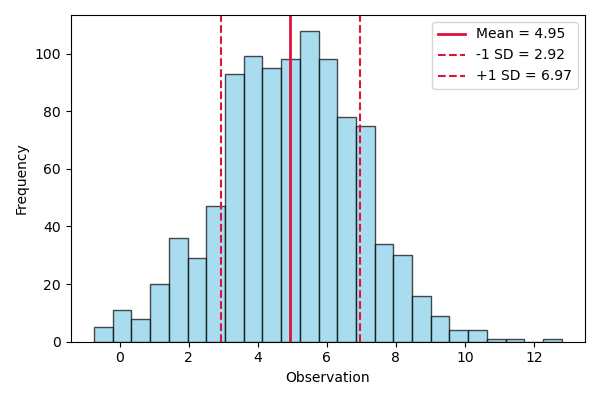
\includegraphics[width=0.7\textwidth]{figures/chapter1/normal_hist.png}
    \caption{Histogram representing the mean and standard deviation for a set of gaussian observations. The read line shows the mean value, representing the central value where the bulk of events lie, and the dotted lines show the standard deviation, as measure of the variability, or how spread the observations are with respect to the mean.}
    \label{fig:histogram1}
\end{figure}

As an exercise, try to compute both the mean and variance for a second sample, let's say

\begin{equation}
\textbf{x}_2 = \{4, 5, 6\} \; . \nonumber
\end{equation}

Buy substituting in the general expressions of $\bar{x}$ and $s^2$ you should get the following results: 

\begin{equation}
\bar{x}_2 = \frac{1}{3} \sum_{i = 1}^{3} x_{i} = \frac{1}{3} (4 + 5 + 6) = 5 \; . \nonumber
\end{equation}

\begin{equation}
s^2_2 = \frac{1}{3 - 1} \sum_{i = 1}^{3} (x_{i} - \bar{x})^{2} = \frac{1}{2} \big((4 - 5)^{2} + (5 - 5)^{2} + (6 - 5)^{2}\big) = \frac{1}{2} (1 + 0 + 1) = 1 \; . \nonumber
\end{equation}

Again, our mean $\bar{x}_2 = 5$ encodes the information about the "central" value, where the bulk of event are, and the variance $s^2_2 = 1$ indicates, as in the previous example, that the elements of the sample $\textbf{x}_2$ are also \textit{one unit} away from the mean.\\

Another useful quantity used to characterize variability is the so called \textit{standard deviation}, which is just the square root of the variance

\begin{equation}
s = \sqrt{\frac{1}{N - 1} \sum_{i = 1}^{N} (x_{i} - \bar{x})^{2}} \; . 
\end{equation}

This is why we have named it in this way, such that $s = \sqrt{s^{2}}$ and our notation remains consistent. Sometimes it is useful to use the standard deviation and sometimes the variance, depending on the question and topic, but as we see they encode essentially the same information.\\

As we said, this was just a warmup example, and we will visit these definitions in further chapters when we introduce the idea of parameter estimation, and we will see in detail different ways to define and interpret them [...]. \\


% Chapter - Probability and random events
\chapter{Probability and random events}

\section{What is probability?}

As already mentioned in the introduction, probability is a branch of mathematics dealing with information and random events. Hence, we could begin by asking, what \textit{are} random events? Random events, also referred to as \textit{stochastic}, are simply processes whose output we \textit{ignore}. As classic examples we could think of tossing coins, rolling dice, or performing some arbitrary measurement. Indeed, the word stochastic comes from no other than the greek word \textgreek{στοχαστικός} (stochastic), which literally means \textit{to guess}. Let's try to briefly introduce the idea of probability, as a quantity that allows as to describe such events and quantify our degree of certainty for a specific result.\\

Let's ask ourselves a the question, what \textit{is} probability in the first place? What do we mean by it and what does it describe? Probability is nothing more, and nothing less, that a \textit{number} we make up, a \textit{quantity} we come up with, to quantify certainty in a process whose outcome we ignore. A number we will use to describe the amount of information we have about a random - or stochastic - event. For simplicity, we can make it range from 0 to 1, in the following way:

\begin{itemize}
\item If I'm sure that some event (A) will never happen, $P(A) = 0$.
\item If I'm sure that some event (A) will always happen,  $P(A) = 1$.
\item For anything in between, if I'm not certain about any of the outcomes, $P(A) \in [0, 1]$.
\end{itemize}

With the symbol $ \in$ we simply denote that $P(A)$ will be a number between 0 and 1. It could also be read as $P(A)$ is \textit{contained} in the interval $[0, 1]$. In all those cases where we are not sure if we will get one result or another, we say that there is a level of \textit{uncertainty}, or \textit{surprise} [...].\\

Let's think on a coins toss, as an example. To model such case, one of the simplest and oldest examples of a stochastic process, we would have two possible outcomes: heads ($H$), and tails ($T$).

\begin{itemize}
\item If I'm sure I will get heads, $P(H) = 1$, and $P(T) = 0$.
\item If I'm sure I will get tails, $P(H) = 0$, and $P(T) = 1$.
\item For anything in between, $P(H) = P(T) = \frac{1}{2}$.
\end{itemize}

The scenarios in which I am certain, of either one case of the other, are clear. But for the third one, where we assign a value to the probability which is not 0 or 1, we should stop for a second. When we say that the probability of getting heads - or tails - in a normal coin that is not biased is $P = \frac{1}{2}$, we are implicitly assuming some things. We implicitly assume that if we repeated the toss many times, half of them we would get one result (e.g., heads), and the other half the remaining result (e.g., tails). This is normally referred to as the \textit{frequentist} definition of probability, because we are defining its value as the ratio of how many times we get a specific result $n$, and the number of total trials $N$. The example of the coin, where we have just two possible results, is what we will call a \textit{Bernoulli} trial, and we will describe it in detail soon, but let's use it now as a prior example to introduce the idea of probability [...] .\\

\begin{equation}
	P(\text{A happening}) = \frac{\text{Number of times A happens}}{\text{Total number of trials}} = \frac{n}{N} \; . \nonumber
\end{equation}

In the case of the coin, if I toss 100 times, and obtain 55 heads against 45 tails, would lead to 

\begin{equation}
	P(\text{H}) = \frac{55}{100} \simeq \frac{1}{2} \; . \nonumber
\end{equation}

Ideally we expect that these frequencies, as we increase the number of repetitions, would approach a perfect $\frac{1}{2}$. We will revisit this concept when we talk about the Law of Large Number and the Central Limit Theorem, in Chapter 3.\\

But this is not the only thing we assume about such a quantity. For probabilities to represent the real behaviour of random processes and information, they must follow another property, called \textit{unitarity}. Unitarity ensures that, if we consider and add up the probabilities for all possible events in a given experiment, we recover the total. That means, at least one of the scenarios will happen.\\

The formal definition of unitarity can be written as follows. Let's denote all possible outcomes of an experiment $x_{1}$, $x_{2}$, ..., $x_{n}$. In the case of coins these will be just $x_{1} = H$, $x_{2} = T$, and with dice, $x_{1} = 1$, $x_{2} = 2$, ..., $x_{6} = 6$. By \textit{unitarity}, we mean that the sum of probabilities of all possible outcomes \text{add up to 1}. \begin{equation}
	\sum_{i = 1}^{n} \; P(x_{i}) = 1
\end{equation}

Indeed, the literal meaning of probability comes from latin \textit{probabilis}. American logician and philosopher Richard Jeffrey, "Before the middle of the seventeenth century, the term "probable" (Latin probabilis) meant just approvable, and was applied in that sense, univocally, to opinion and to action. A probable action or opinion was one such as sensible people would undertake or hold, in the circumstances." However, in legal contexts especially, "probable" could also apply to propositions for which there was good evidence [...].\\

There have been at least two successful attempts to formalize probability, namely the Kolmogorov formulation and the Cox formulation. In Kolmogorov's formulation (see also probability space), sets are interpreted as events and probability as a measure on a class of sets. In Cox's theorem, probability is taken as a primitive (i.e., not further analyzed), and the emphasis is on constructing a consistent assignment of probability values to propositions. In both cases, the laws of probability are the same, except for technical details [...].\\

\newpage

\section{Discrete probability distributions}

So far we have introduced the idea of random events, and the concept of probability as a number to quantify surprise. For our present chapter, we will try to model such stochastic events such that we can make predictions. For that purpose, we will model that probability we just defined to be a descriptive - even better, \textit{predictive} - quantity. Let's begin by saying that not all random phenomena are equal. Hence, a basic way to classify and separate random events, is according to how their probabilities are \textit{distributed}.
 
 \subsection{Bernoulli distribution}

The simplest case we can think of is the \textbf{Bernoulli trial}, named after Swiss mathematician Jacob Bernoulli in late 1600s. A Bernoulli trial is a random experiment with exactly two possible outcomes: \textit{success}, usually labeled as 1, and \textit{failure}, labeled as 0. The probability of success is denoted by $p$, and the probability of failure is $1 - p$.
Mathematically, for a single Bernoulli trial with random variable $x$,

\begin{equation}
P(x = 1) = p \quad \text{and} \quad P(x = 0) = 1 - p,
\end{equation}

where $p \in [0, 1]$. Note that both probabilities do sum 1, and hence if they properly obey the unitarity property. As well, you can see that this is a generalization of the case of the coin, in which the two outcomes had the same probability $p = 0.1$ [...]. Jacob Bernoulli (1655–1705) was one indeed of the pioneers of probability theory. His work \textit{Ars Conjectandi}, published posthumously in 1713, laid the groundwork for the law of large numbers and formalized many concepts still used today.

\begin{figure}[ht]
    \centering
    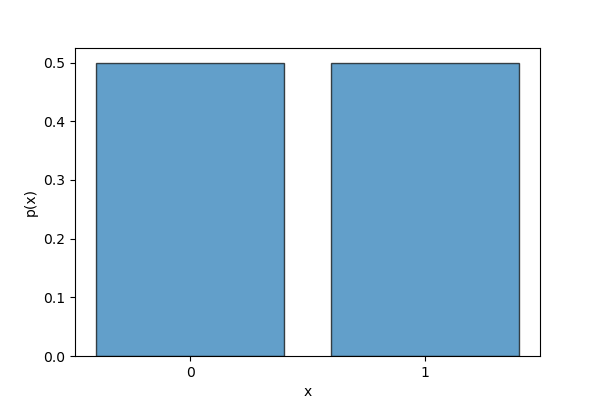
\includegraphics[width=0.7\textwidth]{figures/chapter2/bernoulli.png}
    \caption{Representation of the bernoulli distribution of a random variable $x$, given the total number of trials $n$ and the individual probability of success $p$.}
    \label{fig:bernoulli1}
\end{figure}

\textbf{Example 1}: A fair coin toss is a Bernoulli trial with:

\begin{equation}
p = P(\text{Heads}) = P(\text{Tails}) = 0.5.
\end{equation}

And we can model it as:
\begin{equation}
x = 
\begin{cases}
1 & \text{if Heads} \\
0 & \text{if Tails}
\end{cases}
\end{equation}

Bernoulli trials form the basis for more complex models such as the \textbf{Binomial distribution}, which models the number of successes in a fixed number of independent Bernoulli trials.

\newpage

\subsection{Binomial distribution}
The simplest case of random event we will describe are the so-called \textit{binomial} events. Cases where we make a certain number of measurements $n$, each with two or more possible outcomes, and we want to know the number of successes. For instance, what would be the probability of measuring, or observing, 5 heads if I toss 10 coins? Or what would be the probability of obtaining 5 times a 6, out of a total of 100 dice rolls? In all these cases we will call $x$ the number of successes we want to observe, $n$ the total number of trials, and $p$ the probability of success in each individual trial. The binomial distribution models the number of successes in a fixed number of independent trials, each with the same probability of success. It was developed by Jacob Bernoulli in the 17th century while studying the probability of repeated Bernoulli trials. His work laid the foundation for the Law of Large Numbers.\\

Intuitively, this distribution is useful when considering repeated experiments with two possible outcomes (success or failure). For example, flipping a fair coin multiple times follows a binomial pattern. We will say that the probability of observing $x$ successes in $n$ total tries, given individual probability of success $p$, is given by:
\begin{equation}
    P(x; n, k) = \binom{n}{x} p^x (1-p)^{n-x},
\end{equation}
This is normally referred to as a probability \textit{mass} distribution. The reason for that, as we will discuss later, is to distinguish such events from other types of events called continuous, for which we will define \text{density} distributions. For now, just keep probability mass distribution as a fancy name, or probability distribution, for simplicity. Let's break this expression down in a couple of examples.

\begin{figure}[ht]
    \centering
    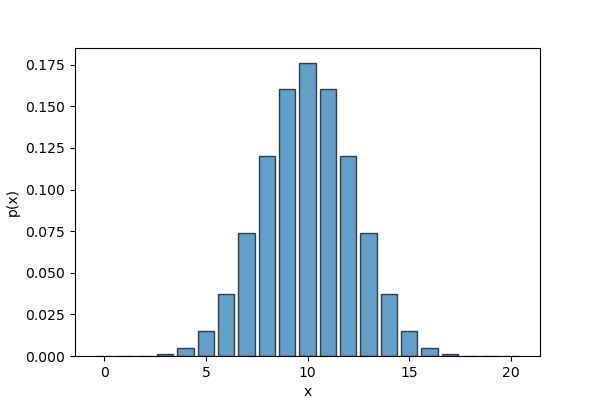
\includegraphics[width=0.7\textwidth]{figures/chapter2/binomial.png}
    \caption{Representation of the binomial distribution of a random variable $x$, given the total number of trials $n$ and the individual probability of success $p$.}
    \label{fig:binomial1}
\end{figure}

\textbf{Example 1:} Suppose we flip a fair coin 5 times ($n=5$) and want to find the probability of getting exactly 3 heads ($p=0.5$):
\begin{align}
    P\bigg(x=5; n = 10; p = \frac{1}{2}\bigg) = &\binom{5}{3} \bigg(\frac{1}{2}\bigg)^3 \bigg(1 - \frac{1}{2}\bigg)^2  \notag \\
    &\binom{5}{3} \bigg(\frac{1}{2}\bigg)^3 \bigg(1 - \frac{1}{2}\bigg)^2  \notag \times 0.25 = 0.3125.
\end{align}\\

\newpage

\subsection{Poisson distribution}
The next kind of random event we will discuss are the \textit{Poisson} distributed, named after the french mathematician Sim\'eon Denis Poisson, who tried to model to events that were random but with a known average rate, such as the number of people crossing a street per day, or the number of customers entering a store, or emails received per hour.
As a note, this distribution was introduced in quite recent times, in the early 19th century to model rare events. It is particularly useful for counting occurrences over a fixed interval of time or space.\\

The probability mass function for observing a number of events $x$ if we know the average rate $\lambda$ is:
\begin{equation}
    P(x; \lambda) = \frac{\lambda^x e^{-\lambda}}{x!},
\end{equation}
Again, let's consider a couple of examples to illustrate Poisson distributed events.

\begin{figure}[ht]
    \centering
    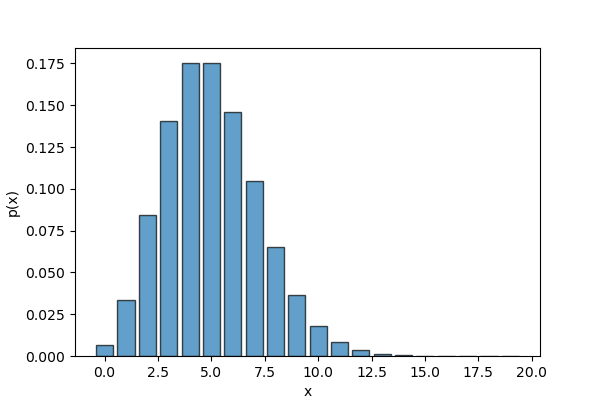
\includegraphics[width=0.7\textwidth]{figures/chapter2/poisson.png}
    \caption{Representation of the Poisson distribution of a random variable $x$, given the number of observations $\lambda$ as a parameter.}
    \label{fig:poisson1}
\end{figure}

\textbf{Example 1:} We would like to know the probability of observing exactly 5 cancer patients in a hospital over a week, if we know the average number ($\lambda = 3$) patients per week.
\begin{equation}
    P(x=5; \lambda = 3) = \frac{3^5 e^{-3}}{5!} = \frac{243 e^{-3}}{120} \approx 0.1008. \notag
\end{equation}\\

\textbf{Example 2:} Let's now ask a similar, but different question. So far, we have only focused on the probability of observing \textit{exactly} one particular outcome. But we could ask as well, what would be the probability observing 5 \textit{or less} cancer patients in that same hospital ($\lambda = 3$) patients per week.
\begin{align}
    P(x \leq 5; \lambda = 3) &= P(x=0; \lambda = 3) + P(x=1; \lambda = 3) + P(x=2; \lambda = 3) \notag \\
    &\quad + P(x=3; \lambda = 3) + P(x=4; \lambda = 3) + P(x=5; \lambda = 3) \notag
\end{align}\\

\newpage

\section{Discrete and continuous}

We will distinguish two main families of random events. These in which the number of possible outcomes is finite, or \textit{countable}, and the ones where the number of outcomes is \textit{uncountable}. The first ones will be named as \textit{discrete} events, while the second are normally referred to as \textit{continuous} [...]. \\

So far we have focused on discrete events, that is, scenarios where the number of possible outcomes was an integer number. Now we will encounter a second family of stochastic processes, the ones we will refer to as continuous. In the discrete case, we were implicitly using the frequentist definition of probability, as a number that represents the ratio of how many times we will observe a particular result, if we endlessly repeat [...].\\

But let's face now a different scenario. What would happen if we try to guess the probability of measuring something which does hace an infinite number of possible outcomes, spread on a continuous range? - e.g., the probability of measuring the height of a person an get 1.75 cm, or the temperature in a room and get 25 degrees, etc. Here we notice that, if we keep the definition of probability we used in the case of the Binomial, the Poisson, etc, we would get something like:

\begin{equation}
P(x = x_{0}) = \frac{\text{number of times I get $x_{0}$}}{\text{number of times I get any other result}}
\end{equation}

Note that now, the possible results are not just 1, 2, ..., n, but actually infinite more and spread over a \textit{continuous} range. The outcome of measuring a temperature could be the $T = 25$ we want, but also $T = 24.999$ and $T = 25.001$, and there are \textit{infinite} other possible results between these two. No matter how precise our measurement devices, are, between any pair of results, we would have an infinite number of cases where we obtain a different result. Hence, applying the frequentist definition of probability would lead to:

\begin{equation}
P(x = x_{0}) = \frac{\text{number of times I get $x_{0}$}}{\text{number of times I get any other result}} = \frac{n}{\infty} = 0
\end{equation}

We would get that the probability of obtaining \textit{any result} would be exactly zero.\\

Let's pause for a moment and think about what happened. At the very beginning of this chapter we said that the quantity $P(x)$ was used to represent information - also certainty, surprise - and computed using the frequentist approach, meaning the \textit{ratio of favorable cases and total cases}. But that was assuming we had a finite set or possibilities, or measure space.

\begin{itemize}
\item Discrete (coins, dice, counting) $\longrightarrow$ finite, \textit{countable} outcomes.
\item Continuous (temperature, energy, concentration, ...) $\longrightarrow$ infinite, \textit{uncountable} outcomes.
\end{itemize}

For such cases we will define a mathematical quantity, similar to that we called probability, which represents analogous information, but considering the fact we are dealing with a continuous event. We will call it \textit{probability density} or simply \textit{density}, and we will denote it with $f(x)$. Note that we can distinguish it from the probability in discrete events $P(x_{i})$, where we used the subscript $x_{i}$ to represent that the random variable could take just a finite set of values ($x_{1}$, $x{2}$, etc).

\begin{itemize}
\item Discrete (coins, dice, counting) $\longrightarrow$ Probability $P(x_{i})$ | $\sum_{i = 1}^{\infty} P(x_{i}) = 1$
\item Continuous (temperature, energy, concentration, ...) $\longrightarrow$ Probability density f(x) | $\int_{i = 0}^{\infty} f(x) dx = 1$
\end{itemize}

In the same way we imposed that probability needs to obey unitarity, we will impose that property in our recently defined probability density $f(x)$. The way we represent the sum for all possible cases in the continuous case, is just imposing that the integral of the function $f(x)$ is 1. This is just an example of \textit{normalization}, that we will explore further in Chapter 4 [...].

\newpage

\section{Continuous probability distributions}

\subsection{Uniform distribution}

The uniform distribution represents events where all outcomes in an interval $[a, b]$ are equally likely [...].\\

The probability of observing a particular result $x$ in a given range $[a, b]$ is:

\begin{equation}
    f(x; a, b) = \frac{1}{b-a}, \quad a \leq x \leq b \; .
\end{equation}

\begin{figure}[ht]
    \centering
    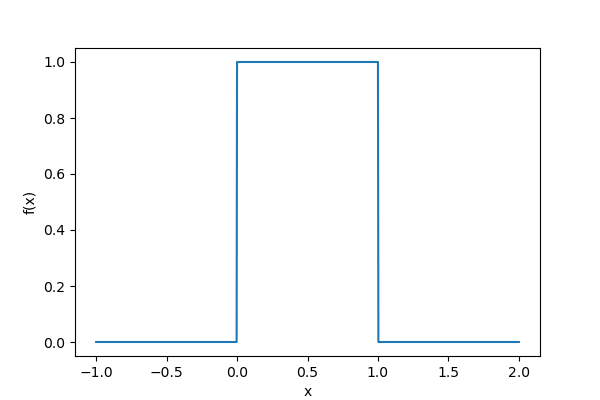
\includegraphics[width=0.7\textwidth]{figures/chapter2/uniform.png}
    \caption{Representation of the uniform distribution of a random variable $x$, given the boundaries $a$, $b$.}
    \label{fig:uniform1}
\end{figure}

\newpage

\subsection{Gaussian distribution}
Introduced by Carl Friedrich Gauss, the normal distribution became central to statistics due to the Central Limit Theorem (CLT). It describes how averages of large samples tend to form a bell-shaped curve. Intuitively, many natural and social phenomena follow a normal distribution, such as human heights and test scores [...].\\

The probability density function is:
\begin{equation}
    f(x; \mu, \sigma) = \frac{1}{\sigma \sqrt{2\pi}} e^{-\frac{(x-\mu)^2}{2\sigma^2}} \; .
\end{equation}

\begin{figure}[ht]
    \centering
    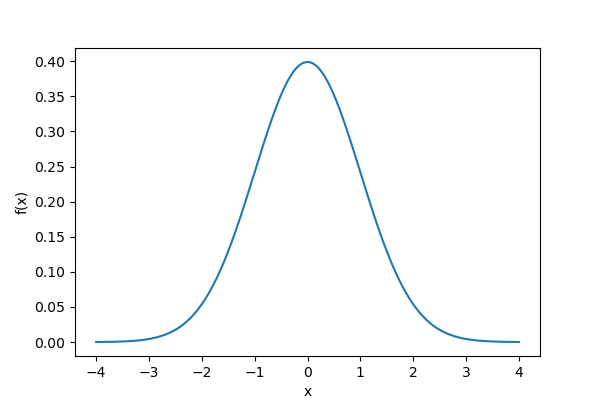
\includegraphics[width=0.7\textwidth]{figures/chapter2/normal.png}
    \caption{Representation of the gaussian distribution of a random variable $x$, given the mean value $\mu$ and standard deviation $\sigma$ parameters.}
    \label{fig:gaussian1}
\end{figure}

\newpage

\subsection{Exponential distribution}
The exponential distribution models waiting times between. Intuitively, it describes situations where the probability of waiting a certain time between events remains constant, such as time between bus arrivals [...].\\

The probability density function is:
\begin{equation}
    f(x; \lambda) = \lambda e^{-\lambda x}, \quad x \geq 0 \; .
\end{equation}

\begin{figure}[ht]
    \centering
    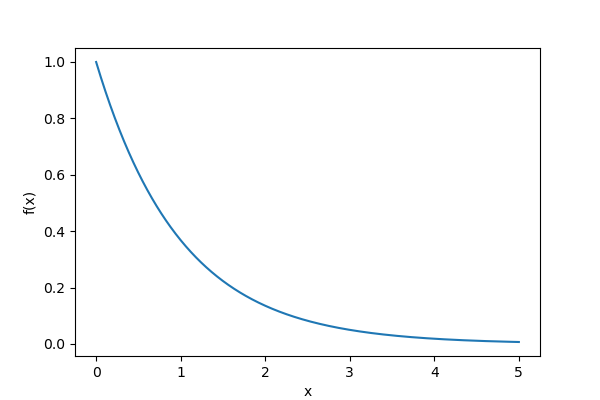
\includegraphics[width=0.7\textwidth]{figures/chapter2/exponential.png}
    \caption{Representation of the exponential distribution of a random variable $x$, given the decay rate $\lambda$.}
    \label{fig:exponential1}
\end{figure}



\newpage

\section*{Exercises}

% Bernoulli trials
\subsection*{Bernoulli trials}

\begin{enumerate}

    \item A single coin is tossed once. What is the probability of getting heads? \\
    
    \textbf{Solution:} \\
    
    In a Bernoulli trial, there are exactly two possible outcomes: success or failure. Here, "success" could mean getting heads, and "failure" means tails. For a fair coin, both outcomes are equally likely. Therefore, the probability \(p\) of success (getting heads) is:
    \[
    p = \frac{\text{Number of favorable outcomes}}{\text{Total number of outcomes}} = \frac{1}{2} = 0.5.
    \]
    So, the probability of getting heads in one toss is \(\boxed{0.5}\).

    \item A biased coin is designed so that the probability of heads is 0.7. What is the probability of getting tails when the coin is tossed once? \\
    
    \textbf{Solution:} \\
    
    Since the coin can only land heads or tails, these two outcomes are complementary events. This means:
    \[
    P(\text{tails}) = 1 - P(\text{heads}).
    \]
    Given \(P(\text{heads}) = 0.7\), we calculate:
    \[
    P(\text{tails}) = 1 - 0.7 = 0.3.
    \]
    Therefore, the probability of getting tails is \(\boxed{0.3}\).

    \item A student answers a true/false question by guessing randomly. What is the probability that the student answers correctly? \\
    
    \textbf{Solution:} \\
    
    A true/false question has two possible answers, only one of which is correct. Since the student guesses without any knowledge, each answer has an equal chance of being selected. Therefore:
    \[
    P(\text{correct}) = \frac{1}{2} = 0.5.
    \]
    So, the probability the student guesses correctly is \(\boxed{0.5}\).
    
\end{enumerate}

% Binomial distribution
\subsection*{Binomial distribution}

\begin{enumerate}

    \item A fair coin is tossed 5 times. What is the probability of getting exactly 3 heads? \\
    
    \textbf{Solution:} \\
    
    When we perform multiple Bernoulli trials (tosses), the number of successes (heads) follows a binomial distribution. The probability mass function (PMF) for the binomial distribution is:
    \[
    P(X = k) = \binom{n}{k} p^k (1-p)^{n-k},
    \]
    where:
    \begin{itemize}
        \item \(n = 5\) is the number of trials (tosses),
        \item \(k = 3\) is the number of successes (heads),
        \item \(p = 0.5\) is the probability of success in each trial.
    \end{itemize}
    First, calculate the binomial coefficient \(\binom{5}{3}\), which counts how many ways to get exactly 3 heads in 5 tosses:
    \[
    \binom{5}{3} = \frac{5!}{3! (5-3)!} = \frac{5 \times 4 \times 3!}{3! \times 2!} = \frac{20}{2} = 10.
    \]
    Now, compute the full probability:
    \[
    P(X=3) = 10 \times (0.5)^3 \times (0.5)^2 = 10 \times 0.125 \times 0.25 = 10 \times 0.03125 = 0.3125.
    \]
    Therefore, the probability of exactly 3 heads in 5 tosses is \(\boxed{0.3125}\) or 31.25\%.

    \item Suppose a basketball player takes 4 free throws, and the probability of scoring each free throw is 0.75. What is the probability that the player scores at least 3 times? \\
    
    \textbf{Solution:} \\
    
    Here:
    \[
    n = 4, \quad p = 0.75, \quad \text{and we want } P(X \geq 3).
    \]
    Since "at least 3 times" means either 3 or 4 successful shots, we calculate:
    \[
    P(X \geq 3) = P(X=3) + P(X=4).
    \]
    Calculate each probability using the binomial formula:
    \[
    P(X=3) = \binom{4}{3} (0.75)^3 (0.25)^1 = 4 \times 0.421875 \times 0.25 = 4 \times 0.10546875 = 0.421875,
    \]
    \[
    P(X=4) = \binom{4}{4} (0.75)^4 (0.25)^0 = 1 \times 0.31640625 \times 1 = 0.31640625.
    \]
    Adding these:
    \[
    P(X \geq 3) = 0.421875 + 0.31640625 = 0.73828125.
    \]
    So, the player has about a \(\boxed{73.8\%}\) chance of scoring at least 3 out of 4 free throws.

    \item In 10 trials, each with a success probability of 0.2, find the probability that there are no successes. \\
    
    \textbf{Solution:} \\
    
    This is the probability of zero successes in 10 independent trials with success probability \(p=0.2\). Using the binomial PMF:
    \[
    P(X=0) = \binom{10}{0} (0.2)^0 (0.8)^{10} = 1 \times 1 \times 0.1073741824 = 0.1073741824.
    \]
    So, the probability of no successes in 10 trials is approximately \(\boxed{0.1074}\) or 10.74\%.
    
\end{enumerate}

% Poisson distribution
\subsection*{Poisson distribution}

\begin{enumerate}

    \item The average number of emails a person receives per hour is 3. What is the probability that exactly 5 emails arrive in one hour? \\
    
    \textbf{Solution:} \\
    
    The Poisson distribution models the probability of a given number of events happening in a fixed interval of time if these events occur with a known constant mean rate and independently of the time since the last event. The PMF of the Poisson distribution is:
    \[
    P(X = k) = \frac{\lambda^k e^{-\lambda}}{k!},
    \]
    where \(\lambda\) is the average number of events per interval and \(k\) is the number of events we want to find the probability for. Here:
    \[
    \lambda = 3, \quad k = 5.
    \]
    Calculate:
    \[
    P(X=5) = \frac{3^5 e^{-3}}{5!} = \frac{243 \times e^{-3}}{120}.
    \]
    Use the approximate value \(e^{-3} \approx 0.04979\):
    \[
    P(X=5) \approx \frac{243 \times 0.04979}{120} = \frac{12.10197}{120} = 0.10085.
    \]
    So, the probability of receiving exactly 5 emails in one hour is approximately \(\boxed{0.1009}\) or 10.09\%.

    \item On average, 2 cars pass a checkpoint per minute. What is the probability that no cars pass in a given minute? \\
    
    \textbf{Solution:} \\
    
    Using Poisson distribution with \(\lambda = 2\) and \(k=0\):
    \[
    P(X=0) = \frac{2^0 e^{-2}}{0!} = e^{-2} \approx 0.1353.
    \]
    Thus, the probability that no cars pass in one minute is about \(\boxed{0.1353}\) or 13.53\%.

    \item Calls arrive at a call center at an average rate of 6 per hour. Find the probability of receiving more than 7 calls in one hour. \\
    
    \textbf{Solution:} \\
    
    Here, \(\lambda = 6\). We want:
    \[
    P(X > 7) = 1 - P(X \leq 7) = 1 - \sum_{k=0}^7 \frac{6^k e^{-6}}{k!}.
    \]
    This cumulative probability \(P(X \leq 7)\) can be found using a Poisson table or a calculator. For example, the sum is approximately 0.8666, so:
    \[
    P(X > 7) = 1 - 0.8666 = 0.1334.
    \]
    Therefore, the chance of more than 7 calls in an hour is roughly \(\boxed{13.34\%}\).
    
\end{enumerate}

% Uniform distribution
\subsection*{Uniform distribution}

\begin{enumerate}

    \item A random variable \(X\) is uniformly distributed between 0 and 10. What is the probability that \(X\) lies between 3 and 7? \\
    
    \textbf{Solution:} \\
    
    The uniform distribution on \([a,b]\) means \(X\) is equally likely to take any value in this interval. The probability density function (pdf) is:
    \[
    f_X(x) = \frac{1}{b-a}, \quad a \leq x \leq b.
    \]
    The probability that \(X\) is between \(c\) and \(d\) (with \(a \leq c < d \leq b\)) is the area under the pdf from \(c\) to \(d\):
    \[
    P(c \leq X \leq d) = \int_c^d f_X(x) \, dx = \frac{d - c}{b - a}.
    \]
    Plug in \(a=0, b=10, c=3, d=7\):
    \[
    P(3 \leq X \leq 7) = \frac{7 - 3}{10 - 0} = \frac{4}{10} = 0.4.
    \]
    Thus, the probability is \(\boxed{0.4}\) or 40\%.

    \item If \(X \sim U(-5,5)\), what is the probability that \(X\) is less than or equal to 0? \\
    
    \textbf{Solution:} \\
    
    The pdf for \(X\) is constant between -5 and 5:
    \[
    f_X(x) = \frac{1}{5 - (-5)} = \frac{1}{10} = 0.1.
    \]
    The probability that \(X \leq 0\) corresponds to the length from -5 up to 0:
    \[
    P(X \leq 0) = \frac{0 - (-5)}{5 - (-5)} = \frac{5}{10} = 0.5.
    \]
    So there is a 50\% chance \(X\) is less than or equal to zero, i.e., \(\boxed{0.5}\).

    \item Find the expected value (mean) and variance of a uniform random variable on \([2,8]\). \\
    
    \textbf{Solution:} \\
    
    For a uniform distribution \(U(a,b)\), the expected value and variance are given by:
    \[
    E[X] = \frac{a + b}{2}, \quad \mathrm{Var}(X) = \frac{(b - a)^2}{12}.
    \]
    Substitute \(a=2\) and \(b=8\):
    \[
    E[X] = \frac{2 + 8}{2} = \frac{10}{2} = 5,
    \]
    \[
    \mathrm{Var}(X) = \frac{(8 - 2)^2}{12} = \frac{6^2}{12} = \frac{36}{12} = 3.
    \]
    So the expected value is \(\boxed{5}\) and the variance is \(\boxed{3}\).
    
\end{enumerate}

% Gaussian distribution
\subsection*{Gaussian distribution}

\begin{enumerate}

    \item A random variable \(X\) is normally distributed with mean \(\mu = 100\) and standard deviation \(\sigma = 15\). Find the probability that \(X\) is less than or equal to 115. \\
    
    \textbf{Solution:} \\
    
    To find this probability, we standardize the variable \(X\) to a standard normal variable \(Z\) which has mean 0 and standard deviation 1. The standardization formula is:
    \[
    Z = \frac{X - \mu}{\sigma}.
    \]
    For \(X = 115\):
    \[
    Z = \frac{115 - 100}{15} = \frac{15}{15} = 1.
    \]
    The probability we want is:
    \[
    P(X \leq 115) = P(Z \leq 1).
    \]
    Using the standard normal distribution table, \(P(Z \leq 1) = 0.8413\).
    
    Therefore, there is an 84.13\% chance that \(X \leq 115\), so the answer is \(\boxed{0.8413}\).

    \item For a standard normal random variable \(Z\), find the probability that \(Z\) lies between -1.5 and 0.5. \\
    
    \textbf{Solution:} \\
    
    The probability that \(Z\) is between two values \(a\) and \(b\) is:
    \[
    P(a \leq Z \leq b) = P(Z \leq b) - P(Z \leq a).
    \]
    Look up the values in the standard normal table:
    \[
    P(Z \leq 0.5) = 0.6915, \quad P(Z \leq -1.5) = 0.0668.
    \]
    So:
    \[
    P(-1.5 \leq Z \leq 0.5) = 0.6915 - 0.0668 = 0.6247.
    \]
    Thus, the probability is approximately \(\boxed{0.6247}\) or 62.47\%.

    \item Find the 90th percentile (also called the 0.9 quantile) of a normal distribution with mean 50 and variance 16. \\
    
    \textbf{Solution:} \\
    
    The standard deviation \(\sigma = \sqrt{16} = 4\). The 90th percentile of a normal distribution corresponds to the value \(x\) such that:
    \[
    P(X \leq x) = 0.9.
    \]
    First, find the corresponding z-score \(z_{0.9}\) for the standard normal distribution. From tables, \(z_{0.9} = 1.2816\).
    Then convert back to the original scale:
    \[
    x = \mu + z_{0.9} \sigma = 50 + 1.2816 \times 4 = 50 + 5.1264 = 55.13.
    \]
    Hence, the 90th percentile is approximately \(\boxed{55.13}\).
    
\end{enumerate}

% Exponential distribution
\subsection*{Exponential distribution}

\begin{enumerate}

    \item The lifetime of a certain type of light bulb follows an exponential distribution with a mean lifetime of 1000 hours. What is the probability that a randomly chosen bulb lasts more than 1200 hours? \\
    
    \textbf{Solution:} \\
    
    The exponential distribution has the probability density function:
    \[
    f_X(x) = \lambda e^{-\lambda x}, \quad x \geq 0,
    \]
    where \(\lambda\) is the rate parameter. The mean lifetime is related to \(\lambda\) by:
    \[
    \text{mean} = \frac{1}{\lambda}.
    \]
    Given the mean is 1000 hours:
    \[
    \lambda = \frac{1}{1000} = 0.001.
    \]
    The probability that the bulb lasts more than \(t\) hours is:
    \[
    P(X > t) = e^{-\lambda t}.
    \]
    For \(t = 1200\):
    \[
    P(X > 1200) = e^{-0.001 \times 1200} = e^{-1.2} \approx 0.3012.
    \]
    Therefore, there is about a \(\boxed{30.12\%}\) chance the bulb lasts longer than 1200 hours.

    \item For the same light bulb, what is the probability that it lasts less than 800 hours? \\
    
    \textbf{Solution:} \\
    
    The probability that the lifetime is less than \(t\) is:
    \[
    P(X < t) = 1 - e^{-\lambda t}.
    \]
    For \(t = 800\):
    \[
    P(X < 800) = 1 - e^{-0.001 \times 800} = 1 - e^{-0.8} \approx 1 - 0.4493 = 0.5507.
    \]
    So, the bulb has a \(\boxed{55.07\%}\) chance of lasting less than 800 hours.

    \item Find the median lifetime of the bulb. \\
    
    \textbf{Solution:} \\
    
    The median \(m\) is the time at which half of the bulbs fail, i.e.:
    \[
    P(X \leq m) = 0.5.
    \]
    Using the cumulative distribution function (CDF):
    \[
    0.5 = 1 - e^{-\lambda m} \implies e^{-\lambda m} = 0.5.
    \]
    Taking natural logarithms:
    \[
    -\lambda m = \ln(0.5) \implies m = -\frac{\ln(0.5)}{\lambda}.
    \]
    Since \(\ln(0.5) = -0.6931\), and \(\lambda = 0.001\):
    \[
    m = \frac{0.6931}{0.001} = 693.1 \text{ hours}.
    \]
    So, the median lifetime is approximately \(\boxed{693.1}\) hours.
\end{enumerate}


% Chapter - Parameter estimation
\chapter{Parameter estimation}

\section{Prediction vs inference}

In the previous chapters we have introduced the mathematical theory of probability. We have developed a series of tools, a \textit{theory}, which enables us to make predictions in stochastic processes. But, contrary to what is normally explain in introductory courses, science is not always headed in the theory - prediction - experiment direction. There can be cases, as we will soon see, where hypothesis are formulated for a given phenomena, and no prediction is made. In such cases, it is from measurement that we will try to see, or \textit{infer} if a given set of assumptions are compatible with the obtained data. Indeed, most modern data analysis and hypothesis testing lie in the \textit{inferential} statistics, rather than \textit{predictive} probability [...].\\

Inference seeks to explain why and how variables relate. The key idea is causality and interpretability: given a some set of observations, inference aims to answer questions such as: Does smoking cause lung cancer, or is the correlation due to other confounding factors? How does an increase in temperature affect ice cream sales? What are the most significant predictors of house prices? The difference between prediction and inference has been a topic of interest in statistics and data science for centuries. While both concepts involve drawing conclusions from data, their goals, methodologies, and historical development differ significantly [...].\\

The roots of inference trace back to classical statistics, particularly the work of Laplace (1749–1827) Gauss (1777–1855), who developed probability theory and the method of least squares. Their work laid the foundation for statistical inference, which aims to understand relationships between variables and make generalizable conclusions about populations from samples. For example, Laplace used probability theory to estimate the population of France, introducing Bayesian inference, which provides a framework for updating beliefs based on observed data. Gauss contributed the normal distribution and least squares estimation, which became essential for making inferences about unknown parameters.

Statistical techniques such as hypothesis testing, confidence intervals, and regression analysis aim to understand and describe these relationships. The emphasis lies on estimating parameters and determining statistical significance rather than simply making accurate predictions. A classic example is Ronald Fisher (1890–1962), who developed maximum likelihood estimation (MLE) to infer parameters of probability distributions. [...].\\

Prediction focuses on accuracy and generalization rather than explaining causality. The goal is to create a model that performs well on new, unseen data, even if the underlying relationships between variables are not fully understood. For example, in modern deep learning, neural networks can recognize faces with high accuracy but offer little interpretability in how they make decisions. Unlike inference, which aims to understand why a pattern exists, prediction is about making the best possible guess given the available data. Focus shifted from understanding relationships to optimizing models that generalize well to unseen data. In 2001, Leo Breiman, in his seminal paper "Statistical Modelling: The Two Cultures," highlighted the distinction, arguing that traditional statistics emphasized inference, whereas modern machine learning prioritized prediction.\\

\section{Parameters and variables}
Another key difference we will discuss now, and quite a subtle one from the mathematical perspective, is that one between a \textit{variable} and a \textit{parameter}. Consider the example of a binomial experiment, e.g. tossing coins and asking for the probability of measuring a specific number of heads. There, we would write it as 

\begin{equation}
    P(x; n, p) = \binom{n}{k} p^x (1-p)^{n-x},
\end{equation}
where $n$ is the number of trials and $p$ is the probability of success.\\

In our previous examples, we have treated just $x$ as our variable of interest, but we could think about P as a function of three independent variables. The number of times we want to observe heads, the total number of trials, and the probability of success for each toss. Normally, we will call \textit{parameters}, to all these variables we will freeze for the purpose of our calculations, and either consider them either known, or fit them from data [...].
 
 \newpage 
 
\section{The Law of Large Numbers}

The Law of Large Numbers (LLN) is one of the fundamental theorems of probability theory. It was first formulated by Jacob Bernoulli in the late 17th century and later refined by other mathematicians, such as Pafnuty Chebyshev. Bernoulli's work aimed to formalize how relative frequencies of events stabilize as the number of trials increases, providing the foundation for statistical inference. LLN plays a crucial role in statistics, finance, and machine learning, ensuring that averages computed from large samples are reliable estimates of expected values.\\

The Law of Large Numbers states that as the sample size increases, the sample mean approaches the expected value. Formally, if $X_1, X_2, \dots, X_n$ are independent and identically distributed (i.i.d.) random variables with expected value $\mathbb{E}[X] = \mu$, then:
\begin{equation}
    \bar{X}_n = \frac{1}{n} \sum_{i=1}^{n} X_i \to \mu \quad \text{as } n \to \infty.
\end{equation}

Consider flipping a fair coin multiple times. The proportion of heads observed converges to 0.5 as the number of flips increases. This illustrates that the observed average stabilizes around the theoretical probability.

\begin{itemize}
    \item \textbf{Weak Law of Large Numbers (WLLN)}: Convergence in probability, i.e., for any $\epsilon > 0$, 
    \begin{equation}
        P(|\bar{X}_n - \mu| \geq \epsilon) \to 0 \quad \text{as } n \to \infty.
    \end{equation}
    \item \textbf{Strong Law of Large Numbers (SLLN)}: Almost sure convergence, i.e.,
    \begin{equation}
        P\left( \lim_{n \to \infty} \bar{X}_n = \mu \right) = 1.
    \end{equation}
\end{itemize}

\begin{figure}[ht]
    \centering
    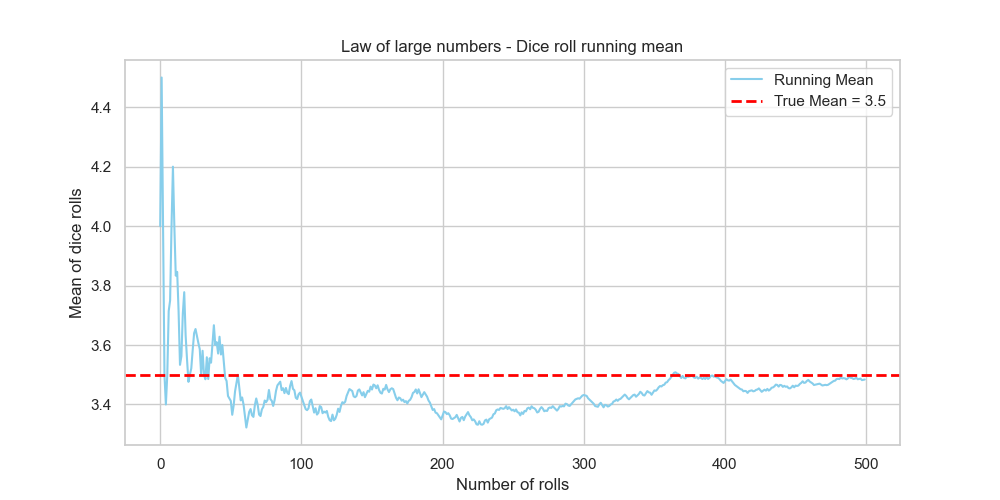
\includegraphics[width=0.7\textwidth]{figures/chapter3/law_large_numbers.png}
    \caption{Representation of the law or large numbers. The sample mean tends to the population mean as the number of rolls $n$ increases.}
    \label{fig:random}
\end{figure}

\textbf{Example:} Suppose we roll a fair six-sided die multiple times. The expected value of a roll is:
\begin{equation}
    \mathbb{E}[X] = \frac{1+2+3+4+5+6}{6} = 3.5.
\end{equation}
As we roll more dice, the sample mean of observed values gets closer to 3.5.

\newpage

\section{The Central Limit Theorem}

The Central Limit Theorem (CLT) was first discovered in the 18th century by Abraham de Moivre and later developed by Pierre-Simon Laplace and Carl Friedrich Gauss. It formalizes the idea that the distribution of sample means tends toward a normal distribution, regardless of the shape of the original population distribution. The CLT is fundamental in inferential statistics, allowing researchers to make predictions and construct confidence intervals for population parameters based on sample data.\\

The Central Limit Theorem states that for a large enough sample size, the sampling distribution of the sample mean follows a normal distribution, regardless of the original population distribution. Formally, if $X_1, X_2, \dots, X_n$ are i.i.d. random variables with mean $\mu$ and variance $\sigma^2$, then the standardized sample mean:
\begin{equation}
    Z = \frac{\bar{X}_n - \mu}{\sigma / \sqrt{n}}
\end{equation}
converges in distribution to a standard normal distribution $\mathcal{N}(0,1)$ as $n \to \infty$.

No matter the shape of the original distribution, when we take many samples and compute their means, the histogram of these sample means will resemble a normal curve as the sample size grows.

\begin{figure}[ht]
    \centering
    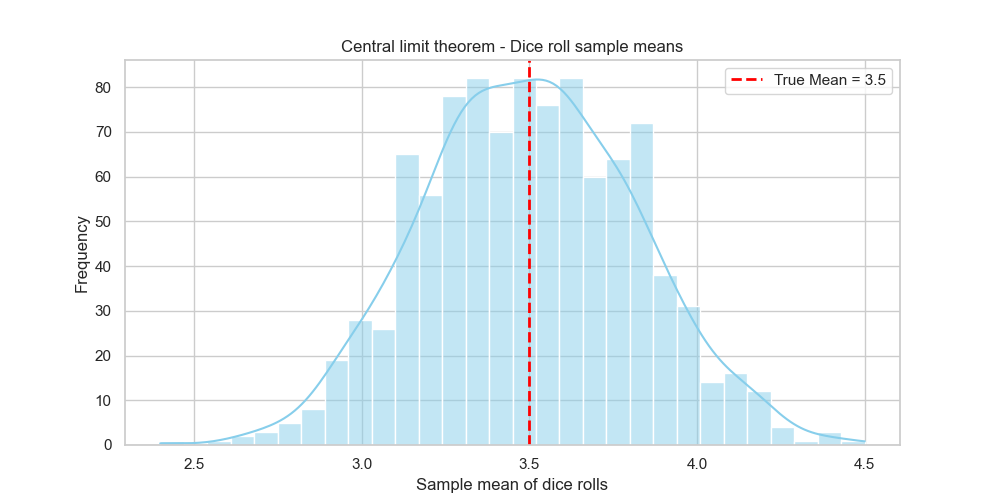
\includegraphics[width=0.7\textwidth]{figures/chapter3/central_limit_theorem.png}
    \caption{Representation of the law or large numbers. The sample mean follows a gaussian distribution as the sample size $n$ increases.}
    \label{fig:random}
\end{figure}

\textbf{Example}: Consider rolling a fair six-sided die multiple times and computing the average outcome for groups of $n$ rolls. As $n$ increases, the distribution of these sample means approaches a normal distribution, centered at $\mu=3.5$.\\

\begin{itemize}
    \item Used in inferential statistics to approximate sampling distributions.
    \item Forms the basis for hypothesis testing and confidence intervals.
    \item Justifies the normality assumption in many statistical models.
\end{itemize}

\newpage

\section{Maximum Likelihood Estimation}

\paragraph{Historical Context:}
Maximum Likelihood Estimation was introduced by the statistician Ronald Fisher in the early 20th century. Fisher’s key insight was that many statistical problems can be solved by choosing the parameters of a model that make the observed data most probable. This approach unified estimation methods and became one of the most fundamental tools in statistics. MLE connects well with probability theory and has wide applications, from genetics to machine learning.

\paragraph{Why Maximum Likelihood?}
In statistics, we often have data generated by some unknown process described by parameters. The goal of MLE is to find the parameter values that best explain the observed data. By defining a likelihood function (the probability of observing the data given parameters), MLE picks the parameters that maximize this function, thus providing the most “likely” explanation.

\paragraph{Applications of MLE:}
MLE is widely used because it produces estimates with good theoretical properties: under mild conditions, MLE estimators are consistent (they get closer to the true value as data grows) and efficient (they have the smallest possible variance among unbiased estimators). It forms the backbone of many models and is implemented in most statistical software.\\

Maximum Likelihood Estimation (MLE) is a cornerstone of modern statistical inference. Developed in the early 20th century by Sir Ronald A. Fisher, MLE provides a systematic framework for estimating the parameters of a probabilistic model. Fisher introduced the method in the 1920s, formalizing it as a rigorous alternative to the method of moments and laying the groundwork for much of classical and modern statistical theory.
MLE has since become one of the most widely used estimation techniques due to its generality, mathematical tractability, and strong theoretical properties. It applies to a broad class of models, including both discrete and continuous distributions, and serves as the basis for many advanced statistical methods, including Generalized Linear Models (GLMs), Bayesian inference (as the likelihood term), and machine learning algorithms.

\subsection{Motivation and intuition}
MLE seeks the parameter $\theta$ that makes the observed data most probable under the assumed model. In other words, it chooses the parameter that maximizes the likelihood function:

\[
L(\theta) = P(X_1 = x_1, \dots, X_n = x_n \mid \theta)
\]

\textbf{Example:} For a Bernoulli distribution with unknown probability $p$, the likelihood of observing a sequence of 0s and 1s is:

\[
L(p) = \prod_{i=1}^{n} p^{x_i}(1-p)^{1 - x_i}
\]

\subsection{The Likelihood and Log-Likelihood functions}

For independent and identically distributed data $X_1, \dots, X_n$ with density or mass function $f(x; \theta)$, the likelihood function is:

\[
L(\theta) = \prod_{i=1}^{n} f(x_i; \theta)
\]

To simplify differentiation, we often use the \textbf{log-likelihood}:

\[
\ell(\theta) = \log L(\theta) = \sum_{i=1}^{n} \log f(x_i; \theta)
\]

To find the MLE $\hat{\theta}$:

\begin{enumerate}
    \item Write down the log-likelihood $\ell(\theta)$.
    \item Take the derivative with respect to $\theta$: $\frac{d\ell}{d\theta}$.
    \item Solve $\frac{d\ell}{d\theta} = 0$ to find critical points.
    \item Check which value maximizes the likelihood (often via the second derivative or boundary checks).
\end{enumerate}

\textbf{Example: Bernoulli MLE}

For $X_i \sim \text{Bernoulli}(p)$,

\[
\ell(p) = \sum_{i=1}^{n} \left[x_i \log(p) + (1 - x_i)\log(1 - p)\right]
\]

Taking derivative:

\[
\frac{d\ell}{dp} = \sum_{i=1}^{n} \left[\frac{x_i}{p} - \frac{1 - x_i}{1 - p}\right] = \frac{\sum x_i}{p} - \frac{n - \sum x_i}{1 - p}
\]

Solving yields:

\[
\hat{p} = \frac{1}{n} \sum_{i=1}^{n} x_i
\]

\subsection{Properties of the MLE}

The importance of MLE lies not only in its general applicability but also in its powerful theoretical properties. 
Under regularity conditions, MLEs are asymptotically optimal estimators in the sense that they:
\begin{itemize}
\item \textbf{Consistency:} $\hat{\theta} \to \theta$ as $n \to \infty$
\item \textbf{Asymptotic Normality:} $\sqrt{n}(\hat{\theta} - \theta) \xrightarrow{d} \mathcal{N}(0, I(\theta)^{-1})$, where $I(\theta)$ is the Fisher information
\item \textbf{Efficiency:} Asymptotically achieves the Cram'er-Rao lower bound
\item \textbf{Invariance:} If $\hat{\theta}$ is the MLE of $\theta$, then $g(\hat{\theta})$ is the MLE of $g(\theta)$ for any differentiable function $g$
\end{itemize}
These properties make MLE a preferred method in both theoretical and applied statistics, especially for large-sample inference. 
In practice, these properties justify the use of MLE even when exact finite-sample distributions are hard to derive.

\subsection{Application to Generalized Linear Models}

Generalized Linear Models (GLMs) are an important class of models that extend linear regression to non-normal response variables by using a link function and a distribution from the exponential family. MLE plays a central role in fitting GLMs because the estimation of the model parameters is achieved by maximizing the likelihood of the observed responses.
For instance, in logistic regression---used for binary outcomes---the log-odds of success is modelled as a linear combination of predictors:\\

\textbf{Example: Logistic Regression}

For binary response data, logistic regression models the log-odds as a linear function of predictors:

\[
\log\left( \frac{p}{1 - p} \right) = \beta_0 + \beta_1 x
\]

MLE is used to estimate the coefficients $\beta_0, \beta_1$ by maximizing the binomial log-likelihood.



\newpage

\section*{Exercises}

% Parameter estimation
\subsection*{Parameter estimation}

\begin{enumerate}

    \item \textbf{Estimating the average height of students:} \\
    A school wants to estimate the average height of its students. They randomly measure the heights of 30 students and calculate the average height to be 160 cm with a sample standard deviation of 10 cm. Estimate the population mean height and explain the meaning of your estimate. \\
    
    \textbf{Solution:} \\
    We have a sample of 30 students with average height \(\bar{x} = 160\) cm. The goal is to estimate the true average height \(\mu\) of all students. The best estimate of \(\mu\) from this sample is simply the sample mean:
    \[
    \hat{\mu} = \bar{x} = 160 \text{ cm}.
    \]
    This means we use 160 cm as our best guess for the average height of the entire student population. Because we only measured 30 students (a sample), this is an estimate, not the exact true mean, but it is the most reasonable value based on the data.

    \item \textbf{Estimating the probability of success in a trial:} \\
    A factory produces light bulbs, and a quality control engineer tests 50 bulbs, finding that 5 bulbs are defective. Estimate the probability that a randomly selected bulb is defective. \\
    
    \textbf{Solution:} \\
    The total bulbs tested: \(n = 50\). Number defective (failures): \(x = 5\). We want to estimate the probability \(p\) of a bulb being defective. The natural estimate is the sample proportion:
    \[
    \hat{p} = \frac{x}{n} = \frac{5}{50} = 0.1.
    \]
    This means we estimate that 10\% of the bulbs are defective. This estimate assumes the sample is representative of the entire production.

    \item \textbf{Estimating the variance of daily sales:} \\
    A store records the number of sales for 7 days as: 20, 22, 18, 25, 24, 20, 19. Estimate the variance of daily sales. \\
    
    \textbf{Solution:} \\
    First, find the sample mean:
    \[
    \bar{x} = \frac{20 + 22 + 18 + 25 + 24 + 20 + 19}{7} = \frac{148}{7} \approx 21.14.
    \]
    Next, calculate the squared deviations from the mean:
    \[
    (20 - 21.14)^2 = 1.30, \quad (22 - 21.14)^2 = 0.74, \quad (18 - 21.14)^2 = 9.86,
    \]
    \[
    (25 - 21.14)^2 = 14.86, \quad (24 - 21.14)^2 = 8.18, \quad (20 - 21.14)^2 = 1.30, \quad (19 - 21.14)^2 = 4.58.
    \]
    Sum of squared deviations:
    \[
    S = 1.30 + 0.74 + 9.86 + 14.86 + 8.18 + 1.30 + 4.58 = 40.82.
    \]
    The sample variance (unbiased estimator) is:
    \[
    s^2 = \frac{S}{n-1} = \frac{40.82}{6} \approx 6.80.
    \]
    So, the estimated variance of daily sales is \(\boxed{6.80}\).

\end{enumerate}

% Central limit theorem
\subsection*{Central limit theorem}

\begin{enumerate}

    \item \textbf{Average weight of apples:} \\
    Suppose the weight of apples in an orchard has an unknown distribution with mean 150 grams and standard deviation 20 grams. A random sample of 36 apples is taken. What is the approximate probability that the average weight of these apples is between 145 and 155 grams? \\
    
    \textbf{Solution:} \\
    Even if the original weight distribution is unknown, the Central Limit Theorem (CLT) tells us that the sampling distribution of the sample mean \(\bar{X}\) for a sample size \(n=36\) is approximately normal with:
    \[
    \mu_{\bar{X}} = \mu = 150, \quad \sigma_{\bar{X}} = \frac{\sigma}{\sqrt{n}} = \frac{20}{\sqrt{36}} = \frac{20}{6} = 3.33.
    \]
    We standardize the bounds:
    \[
    Z_1 = \frac{145 - 150}{3.33} = \frac{-5}{3.33} \approx -1.5,
    \]
    \[
    Z_2 = \frac{155 - 150}{3.33} = \frac{5}{3.33} \approx 1.5.
    \]
    Using standard normal tables:
    \[
    P(-1.5 \leq Z \leq 1.5) = P(Z \leq 1.5) - P(Z \leq -1.5) = 0.9332 - 0.0668 = 0.8664.
    \]
    So, there is about an 86.64\% chance that the sample average weight is between 145 and 155 grams.

    \item \textbf{Average waiting time at a bus stop:} \\
    The waiting time for buses is skewed but has mean 10 minutes and standard deviation 5 minutes. If 50 people independently measure their waiting times. What is the approximate probability that the average waiting time of these 50 people is more than 12 minutes? \\
    
    \textbf{Solution:} \\
    By the CLT, the sample mean \(\bar{X}\) is approximately normal with:
    \[
    \mu_{\bar{X}} = 10, \quad \sigma_{\bar{X}} = \frac{5}{\sqrt{50}} = \frac{5}{7.07} \approx 0.707.
    \]
    Standardize 12:
    \[
    Z = \frac{12 - 10}{0.707} = \frac{2}{0.707} \approx 2.83.
    \]
    Look up the standard normal table:
    \[
    P(Z > 2.83) = 1 - P(Z \leq 2.83) = 1 - 0.9977 = 0.0023.
    \]
    So, there is a 0.23\% chance that the average waiting time exceeds 12 minutes.

    \item \textbf{Average number of daily customers:} \\
    A store knows the daily number of customers varies widely, with mean 100 and standard deviation 30. If we take a random sample of 64 days, what is the probability that the average customers per day is between 95 and 105? \\
    
    \textbf{Solution:} \\
    Sample mean distribution approximately normal with:
    \[
    \mu_{\bar{X}} = 100, \quad \sigma_{\bar{X}} = \frac{30}{\sqrt{64}} = \frac{30}{8} = 3.75.
    \]
    Standardize the bounds:
    \[
    Z_1 = \frac{95 - 100}{3.75} = -1.33, \quad Z_2 = \frac{105 - 100}{3.75} = 1.33.
    \]
    From standard normal tables:
    \[
    P(-1.33 \leq Z \leq 1.33) = 0.9082 - 0.0918 = 0.8164.
    \]
    Therefore, there's about an 81.64\% chance the sample mean is between 95 and 105 customers.

\end{enumerate}

% Law of large numbers
\subsection*{Law of large numbers}

\begin{enumerate}

    \item \textbf{Coin toss average:} \\
    You toss a fair coin many times, recording the proportion of heads. According to the Law of Large Numbers (LLN), what happens to this proportion as the number of tosses increases? Explain in simple terms. \\
    
    \textbf{Solution:} \\
    The LLN states that as the number of tosses \(n\) becomes very large, the sample proportion of heads will get closer and closer to the true probability \(p = 0.5\). In simple terms, if you toss the coin only a few times, the proportion of heads may be very different from 0.5, but if you toss it thousands of times, the proportion of heads will be almost exactly 50\%. This happens because random fluctuations average out over many trials.

    \item \textbf{Average daily sales convergence:} \\
    A store records daily sales, which vary widely, with an unknown distribution but average 200 sales/day. How does the Law of Large Numbers help the store owner understand the average sales if they calculate the average over many days? \\
    
    \textbf{Solution:} \\
    The LLN guarantees that if the store owner calculates the average sales over a large number of days, the average they get will be very close to the true average sales per day (which is 200). So, even if sales fluctuate a lot from day to day, the long-term average will stabilize and become predictable when many days are included.

    \item \textbf{Estimating average waiting time at a clinic:} \\
    The waiting time for patients varies, but the average is 30 minutes. If a patient measures their waiting time many times over different visits, what does the Law of Large Numbers say about the average of their measured times? \\
    
    \textbf{Solution:} \\
    The LLN tells us that as the patient records more and more waiting times, the average of these recorded times will get closer and closer to 30 minutes. So, although a single visit may have a short or long wait, the average wait over many visits will reliably approach the true average.

\end{enumerate}

\newpage

% Maximum likelihood estimation
\subsection*{Maximum likelihood estimation}

\begin{enumerate}

	\item \textbf{Exercise 1: MLE for a Coin Toss}
	You toss a coin 10 times and observe 7 heads. Using MLE, estimate the probability of heads $p$.

	\subsubsection*{Solution}
	Let $p$ be the probability of heads. The likelihood function for 7 heads out of 10 tosses (binomial distribution) is:
	\[
	L(p) = \binom{10}{7} p^7 (1-p)^3
	\]

	Since the binomial coefficient does not depend on $p$, maximize:
	\[
	\ell(p) = p^7 (1-p)^3
	\]

	To maximize $\ell(p)$, it is easier to maximize the log-likelihood:
	\[
	\log \ell(p) = 7 \log p + 3 \log (1-p)
	\]

	Take derivative w.r.t. $p$ and set to zero:
	\[
	\frac{7}{p} - \frac{3}{1-p} = 0
	\Rightarrow 7(1-p) = 3p
	\Rightarrow 7 - 7p = 3p
	\Rightarrow 7 = 10p
	\Rightarrow p = \frac{7}{10} = 0.7
	\]

	Thus, the MLE estimate for the probability of heads is 0.7, matching the observed proportion.

	\item \textbf{Exercise 2: MLE for Exponential Distribution}
	Suppose the time between phone calls follows an exponential distribution with unknown rate $\lambda$. You observe waiting times: 2, 3, 1. Find the MLE for $\lambda$.

	\subsubsection*{Solution}
	The exponential distribution’s PDF is:
	\[
	f(t|\lambda) = \lambda e^{-\lambda t}, \quad t \geq 0
	\]

	The likelihood for data points $t_1, t_2, t_3$ is:
	\[
	L(\lambda) = \prod_{i=1}^3 \lambda e^{-\lambda t_i} = \lambda^3 e^{-\lambda \sum t_i}
	\]

	Log-likelihood:
	\[
	\log L(\lambda) = 3 \log \lambda - \lambda \sum t_i
	\]

	Derivative w.r.t. $\lambda$:
	\[
	\frac{3}{\lambda} - \sum t_i = 0 \implies 3 = \lambda \sum t_i \implies \hat{\lambda} = \frac{3}{\sum t_i}
	\]

	Calculate sum of times:
	\[
	2 + 3 + 1 = 6
	\]

	Thus,
	\[
	\hat{\lambda} = \frac{3}{6} = 0.5
	\]

	So, the MLE estimate for $\lambda$ is 0.5 calls per unit time.

	\item \textbf{Exercise 3: MLE for Normal Distribution Mean}
	You have data points $x = \{4, 5, 6\}$ from a normal distribution with unknown mean $\mu$ and known variance $\sigma^2 = 1$. Find the MLE for $\mu$.

	\subsubsection*{Solution}
	The likelihood is:
	\[
	L(\mu) = \prod_{i=1}^3 \frac{1}{\sqrt{2\pi}} e^{-\frac{(x_i - \mu)^2}{2}}
	\]

	Log-likelihood (ignoring constants):
	\[
	\log L(\mu) = -\frac{1}{2} \sum_{i=1}^3 (x_i - \mu)^2
	\]

	To maximize, minimize the sum of squared differences:
	\[
	\frac{d}{d\mu} \left( \sum (x_i - \mu)^2 \right) = 0
	\]

	\[
	-2 \sum (x_i - \mu) = 0 \Rightarrow \sum x_i = 3 \mu \Rightarrow \mu = \frac{1}{3} \sum x_i
	\]

	Calculate:
	\[
	\mu = \frac{4 + 5 + 6}{3} = \frac{15}{3} = 5
	\]

	The MLE estimate for the mean is 5, which is the sample average.

\end{enumerate}



% Chapter - Introduction to hypothesis testing
\chapter{Introduction to hypothesis testing}

\section{Prediction vs inference}

The philosophical divide between inference and prediction has deep roots in the evolution of scientific reasoning. Inference, rooted in the classical traditions of epistemology, seeks to illuminate the underlying structure or cause of observed data. It asks, fundamentally, why we see what we do, invoking theories, latent mechanisms, and parameters that might explain the phenomena. Prediction, by contrast, is more agnostic to explanation and more utilitarian: it is concerned with what will happen next. The rise of probabilistic models in the 20th century made it possible to quantify uncertainty in both tasks, but their goals remain distinct. Inference aims to learn about the data-generating process; prediction aims to accurately forecast future observations, regardless of the process's inner workings \cite{student1908}, \cite{fisher1925},  \cite{fisher1935}.\\

This distinction becomes particularly important in statistical modeling. Predictive models, such as those deployed in machine learning, are often evaluated by their performance on unseen data, with little regard for the interpretability of parameters. Inference, however, thrives on interpretable structure—effect sizes, confidence intervals, causal assumptions—offering insights that extend beyond mere forecasting. Yet the two are not mutually exclusive: many contemporary methods, especially in Bayesian statistics, attempt to harmonize prediction and inference within unified frameworks. Still, when decisions hinge on understanding causation or evaluating mechanisms—as in medicine, economics, or the social sciences—inference retains a privileged role.\\

\begin{figure}[ht]
    \centering
    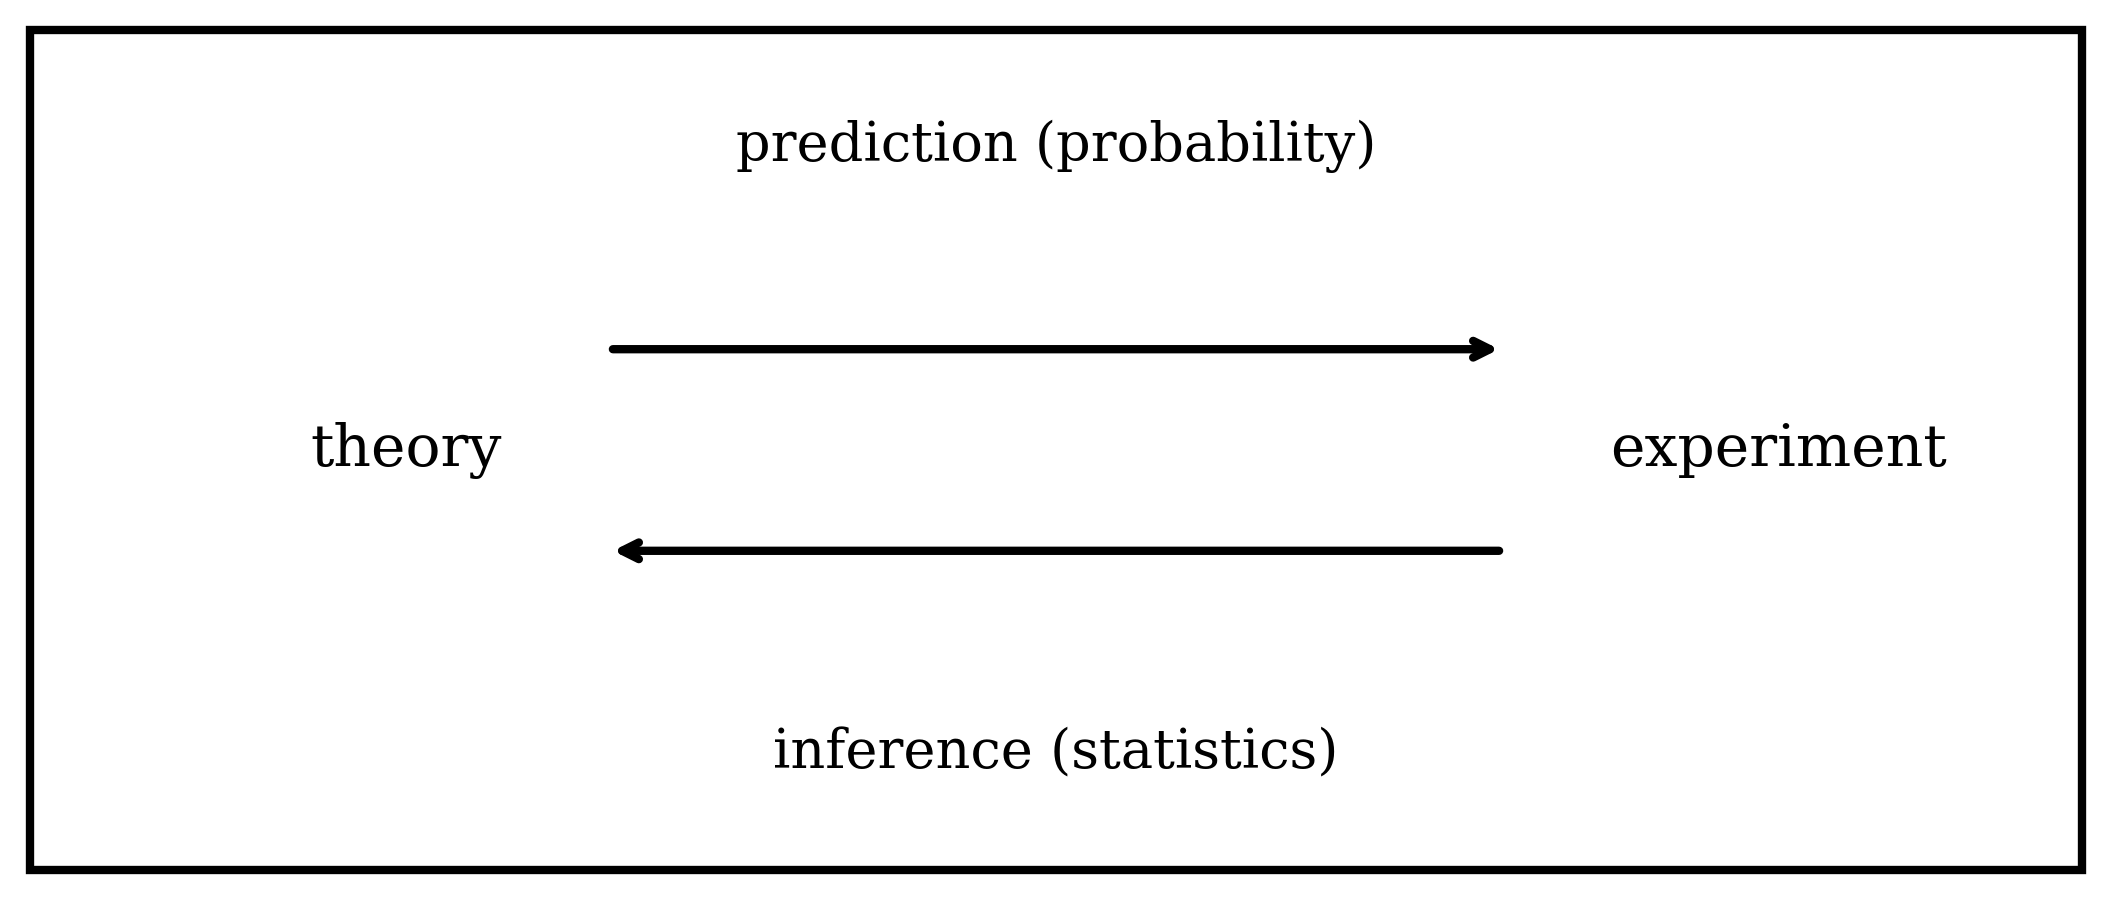
\includegraphics[width=0.6\textwidth]{figures/chapter4/probability_vs_statistics.png}
    \caption{Representation of the predictive (from theory to experimental verification) and inferential (from data to underlying truth, descriptive and hypothesis testing) approaches to probability and statistics \cite{pearson1900}.}
    \label{fig:prob_vs_stats1}
\end{figure}

Within this context, hypothesis testing emerges as a formal tool to carry out inference under uncertainty. Popularized in the early 20th century by Ronald A. Fisher and later formalized by Jerzy Neyman and Egon Pearson, hypothesis testing provides a structured way to assess whether observed data is consistent with a particular theoretical claim. At its core, the method pits a "null" hypothesis (typically representing chance or no effect) against an "alternative," calculating the probability of observing data as extreme as ours under the null. While often misused or misinterpreted, hypothesis testing remains foundational in the sciences—offering a bridge between data and theory, between the probabilistic world of prediction and the explanatory realm of inference \cite{fisher1925}, \cite{fisher1935}.\\

In the previous chapters we have introduced the mathematical theory of probability. That is, we have developed a series of tools, a \textit{theory}, which enables us to make predictions in stochastic processes. But, contrary to what is normally explain in introductory courses, science is not always headed in the theory - first - and experiment - after - direction. There can be cases, as we will soon see, where hypothesis are formulated for a given phenomena, and no prediction is made. In such cases, it is from measurement that we will try to see, or \textit{infer} if our hypothesis are compatible with given data. Indeed, most modern data analysis and hypothesis testing lie in the inferential statistics, rather than predictive probability.

\section{Hypothesis, significance, p-values}
The term \textit{hypothesis testing} is usually used to refer a broad set of tools addressing parameter estimation, inference, and various exploratory analysis on random measurements and observations. It was first coined by British mathematicians Pearson and Fisher [...] in early XX\textsuperscript{th} century. In the last decades, hypothesis testing, hypothesis test, statistical inference - sometimes referred to as  exploratory analysis - has gained popularity and become one of the standards in most experimental sciences, given the automatization of experiments and the large amounts of data available.\\

Once we have covered the idea of parameter estimation, sample distributions, and the idea of estimators, we will now formulate hypothesis on the true - \textit{unkwnown} - parameters, and then build \textit{statistic tests} to quantify how far - or close - are these hypothesized values from the observed - experimental, sample - values. And finally, we will quantify how certain we are about the values obtained - how \textit{significant} they are - computing the \textit{p-value}, standing from Pearson value.\\ The general approach we will follow, regardless of the kind of question we are after and the observations made, can be summarized as follows:

\begin{itemize}
\item Formulate \textit{null} hypothesis $H_0$ and \textit{alternative} hypothesis $H_1$ about the \textit{true} - \textit{population} parameters, generally for the mean or variance, \textit{prior to experiment}.
\item Collect data, make observations, make measurements.
\item Compute \textit{informative quantities} from our observed values, normally referred to as \textit{statistics}, or \textit{statistic tests}
\item Compute p-value, probability of \textit{given the null hypothesis was true} obtained a value at leas as extreme as the one we obtained for our statistic test.
\item Accept or reject the null hypothesis, based on the p-value.
\end{itemize}

\newpage

\section{Statistical tests: some examples}

\subsection{Compare sample mean with hypothesized value - One sample t-test}

The t test, a cornerstone of inferential statistics, emerged from a union of practical necessity and mathematical ingenuity in the early 20th century. Its origin is entwined with the world of brewing: William Sealy Gosset, a statistician employed by the Guinness Brewery in Dublin, devised the method to address the problem of making reliable inferences from small sample sizes—a common challenge in quality control. Because Guinness forbade its employees from publishing research, Gosset adopted the pseudonym “Student,” and the t test entered the statistical canon as “Student’s t test.” Far from being a mere curiosity, this test helped lay the foundation for modern statistical thinking, offering a systematic way to evaluate whether observed differences could be attributed to chance \cite{student1908}.\\

Contextually, the t test emerged during a period of growing interest in the mathematical modeling of uncertainty. While the 19th century had seen the establishment of probability theory and the development of the normal distribution by figures like Gauss and Laplace, it was not until the early 20th century that statisticians began to grapple earnestly with small samples and experimental variability. Gosset’s innovation came at a time when the rigor of scientific inquiry was undergoing transformation—where laboratory science, agricultural experimentation, and industrial quality control all demanded more precise methods of inference. The t distribution, with its heavier tails than the normal distribution, aptly modeled the added uncertainty inherent in small datasets, providing a safeguard against overconfidence in inferences drawn from limited observations.\\

In the broader sweep of statistical development, the t test exemplifies the bridging of theoretical elegance and empirical utility. It stands as a testament to the democratization of statistical methods—making it feasible for practitioners across disciplines to assess hypotheses without the need for large-scale experimentation. Its adaptability, whether in comparing means between two groups or assessing paired observations, has ensured its enduring presence in the researcher’s toolkit. Over a century later, the t test remains not merely a relic of an industrial past but a living method, still invoked in clinical trials, psychological studies, and countless scientific explorations, bearing with it both the legacy of its creator and the evolving rigor of modern analysis.\\

\begin{figure}[ht]
    \centering
    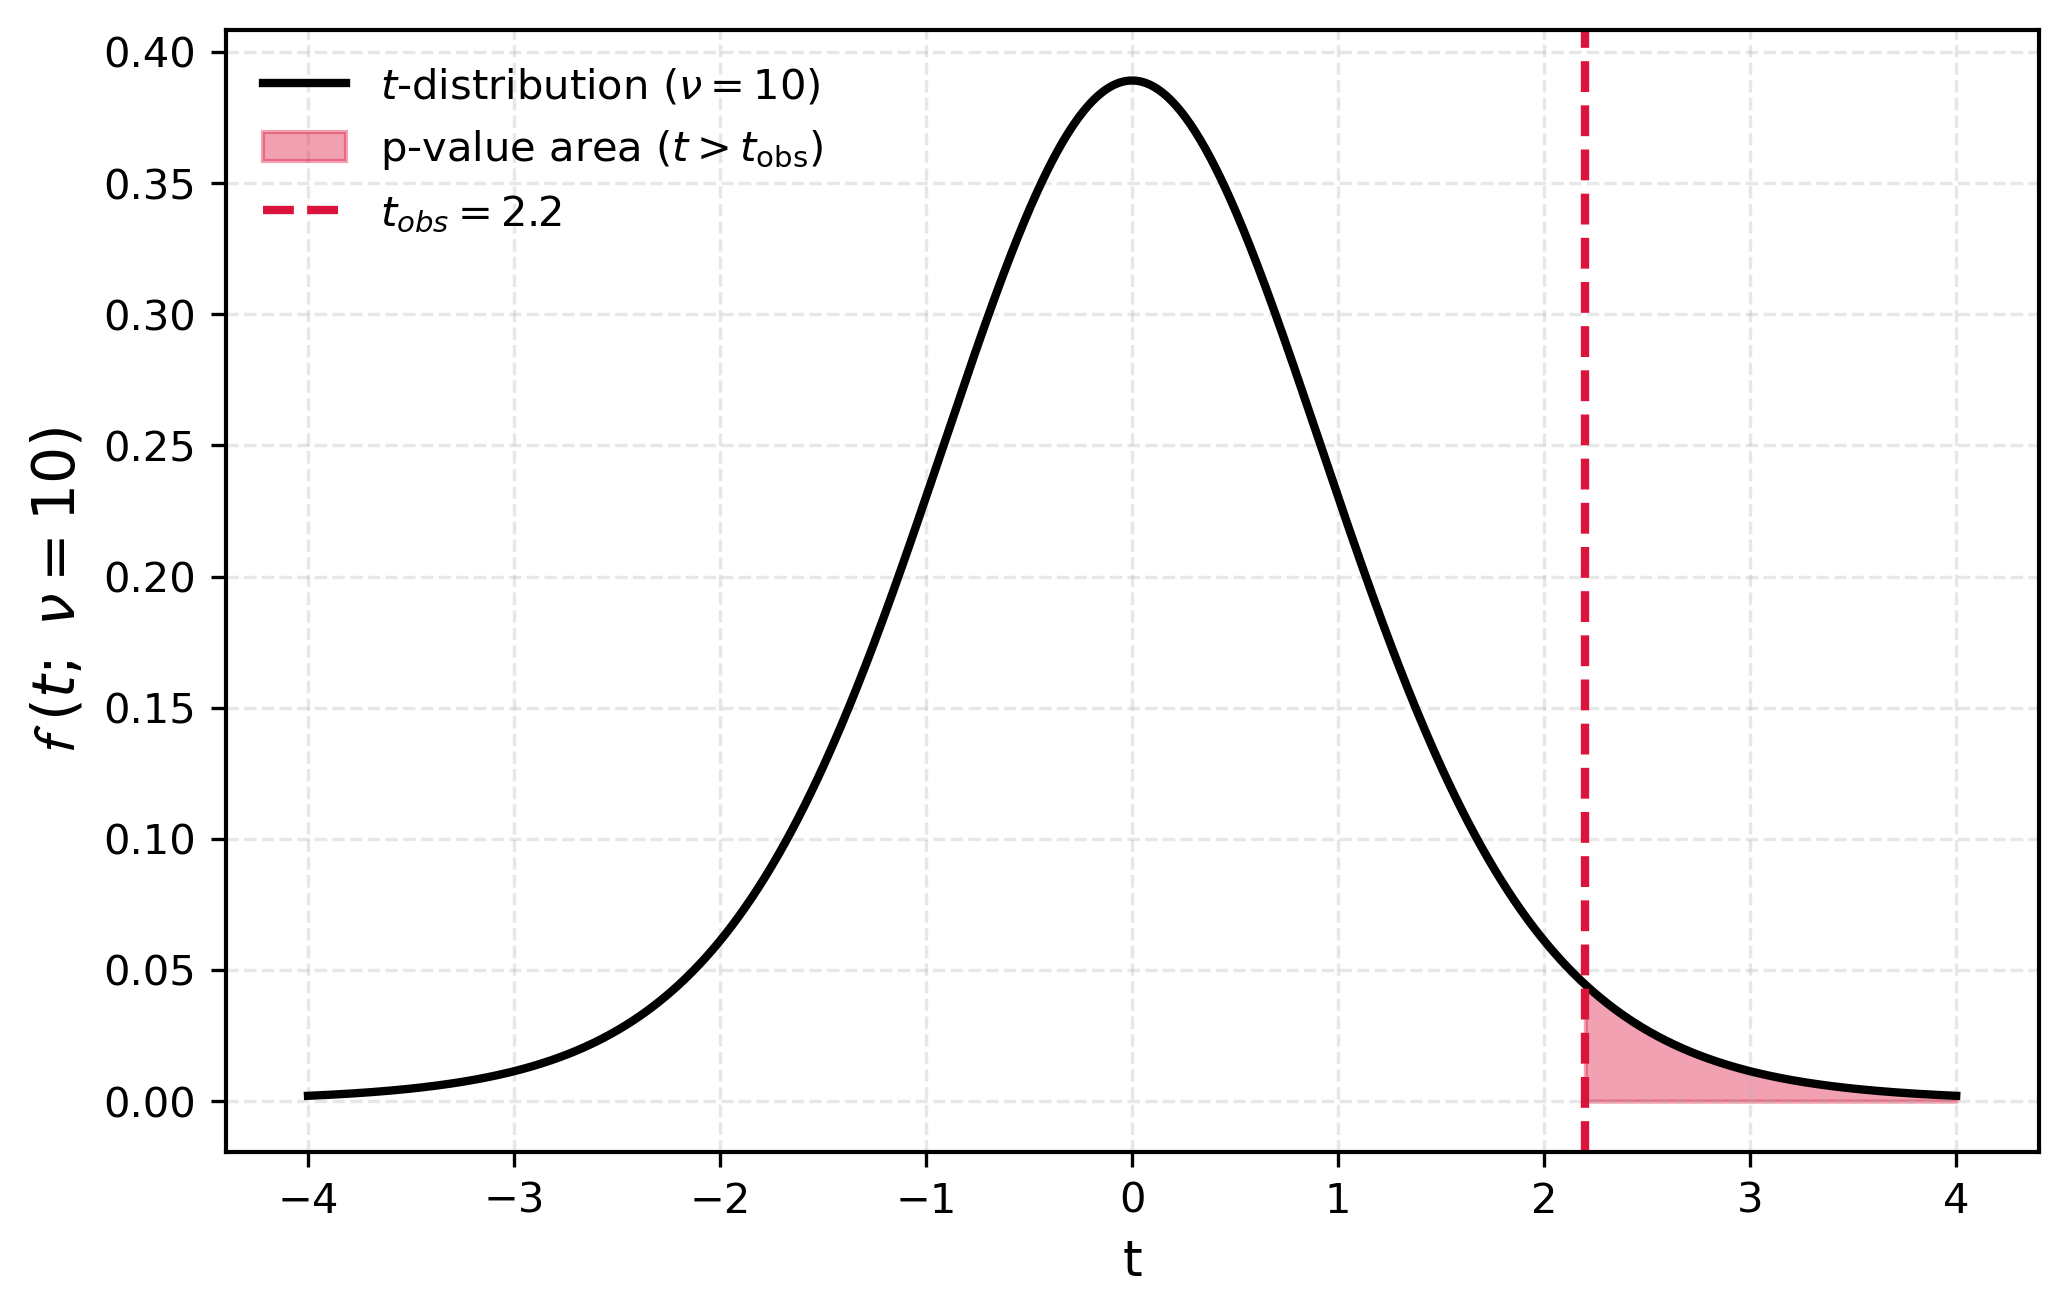
\includegraphics[width=0.7\textwidth]{figures/chapter4/t_test_1_sample_p_one_tailed.png}
    \caption{Representation of the t statistic, following the Student's t distribution, for a particular value of the degrees of freedom ($\nu = 10$). The integral of the shadowed area represents the \textit{1-sided}, or \textit{1-tailed} p-value, as the probability of obtaining a result \textit{at least as extreme} as the one obtained $t_{obs}$.}
    \label{fig:t_test1}
\end{figure}

The student's t is used to compare the sample mean $\bar{x}$ to ha hypothesized value $\mu$. It assumes that the sample data are drawn from a normally distributed population, hence it is an example of a \textit{parametric} test. We will discuss more about parametric and non-parametric observations, and how to test for normality further in the chapter. The test statistic is given by:
\[
    t = \frac{\bar{x} - \mu}{s / \sqrt{n}},
\]

where $\bar{x}$ is the sample mean, $\mu$ is the population mean, $s$ is the sample standard deviation, and $n$ is the sample size. It is built in such a way that, as the sample mean $\bar{x}$ gets closer to the hypothesized value $\mu$, the $t$-variable approaches zero.\\

Then, given some data was observed and and we obtained a specific value for our t - let's call it \textit{t obs}, to compute a p-value we just need to compute what was the probability of that particular value. To do that, we just recall our t variable was indeed a random variable depending on our random observations, which produced some random sample mean and variance, and some degrees of freedom $n - 1$
\[
p = P\left(t > t obs \right) = 2 \cdot \int_{|t|}^{\infty} f_{T_{n-1}}(x)\,dx = 2 \cdot \left[1 - F_{T_{n-1}}(|t|)\right]
\]

\subsection*{The t distribution}

Being $f_{T_{n-1}}$ the PDF of the t variable, the \textit{Student's t distribution} with $n - 1$ degrees of freedom, and $F_{T_{n-1}}$ the corresponding cumulative distribution, as we discussed in chapter 2 [...]. Here, we are computing the probability of t being greater than the one we obtained, and we do that just by integrating the t-distribution [...]. Note that here we are computing a 2-sided p-value, hence te factor 2 at the beginning. 

Given a sample \( X_1, \ldots, X_n \sim \mathcal{N}(\mu, \sigma^2) \), the one-sample \textit{t}-statistic is defined as:
\[
t = \frac{\bar{X} - \mu_0}{S / \sqrt{n}}
\]
where \( \bar{X} \) is the sample mean, \( S \) is the sample standard deviation, and \( \mu_0 \) is the hypothesized population mean.

Under the null hypothesis \( H_0: \mu = \mu_0 \), the statistic follows a Student's \textit{t}-distribution with \( n-1 \) degrees of freedom:
\[
t \sim t_{n-1}
\]
The probability density function (PDF) of the \textit{t}-distribution with \( \nu \) degrees of freedom is:
\[
f(t) = \frac{\Gamma\left(\frac{\nu+1}{2}\right)}{\sqrt{\nu \pi} \, \Gamma\left(\frac{\nu}{2}\right)} \left(1 + \frac{t^2}{\nu}\right)^{-\frac{\nu+1}{2}}
\]
Distribution and computation of the p-value as defined above.

\newpage

\subsection{Compare sample means of two independent groups - Two sample t-test}

The two-sample t test represents a natural extension of Student’s original formulation, expanding its reach from single-sample inference to the comparison of two independent groups. This test seeks to determine whether the means of two populations differ significantly, based on sample data—often drawn from experimental and observational studies. It operates under the assumption that the underlying distributions are approximately normal and that the variances between groups are equal or at least comparable, though variants like Welch’s t test have relaxed these conditions. The test statistic itself balances the observed difference in means against the pooled standard error, weighing signal against noise \cite{student1908}.\\

The historical roots of the two-sample t test are intertwined with the rise of controlled experimentation in the biological and social sciences during the early to mid-20th century. Ronald Fisher, Jerzy Neyman, and Egon Pearson contributed to formalizing the logic of hypothesis testing, and the t test became a practical tool within this growing paradigm. Its popularity grew not merely because it was mathematically sound, but because it was accessible—a concise, interpretable method for testing simple but essential questions in science: does treatment differ from control, or is an observed effect more than a fluke?\\

Even in today’s data-rich landscape, the two-sample t test remains remarkably resilient. Its conceptual clarity and computational simplicity make it a first recourse in evaluating differences between two conditions, from clinical trials comparing drug efficacies to educational studies assessing learning interventions. In many ways, it is the distilled essence of statistical thinking: discerning pattern from randomness, while acknowledging uncertainty. Its elegance lies not in its complexity, but in its ability to render the ordinary rigorously meaningful.\\

\begin{figure}[ht]
    \centering
    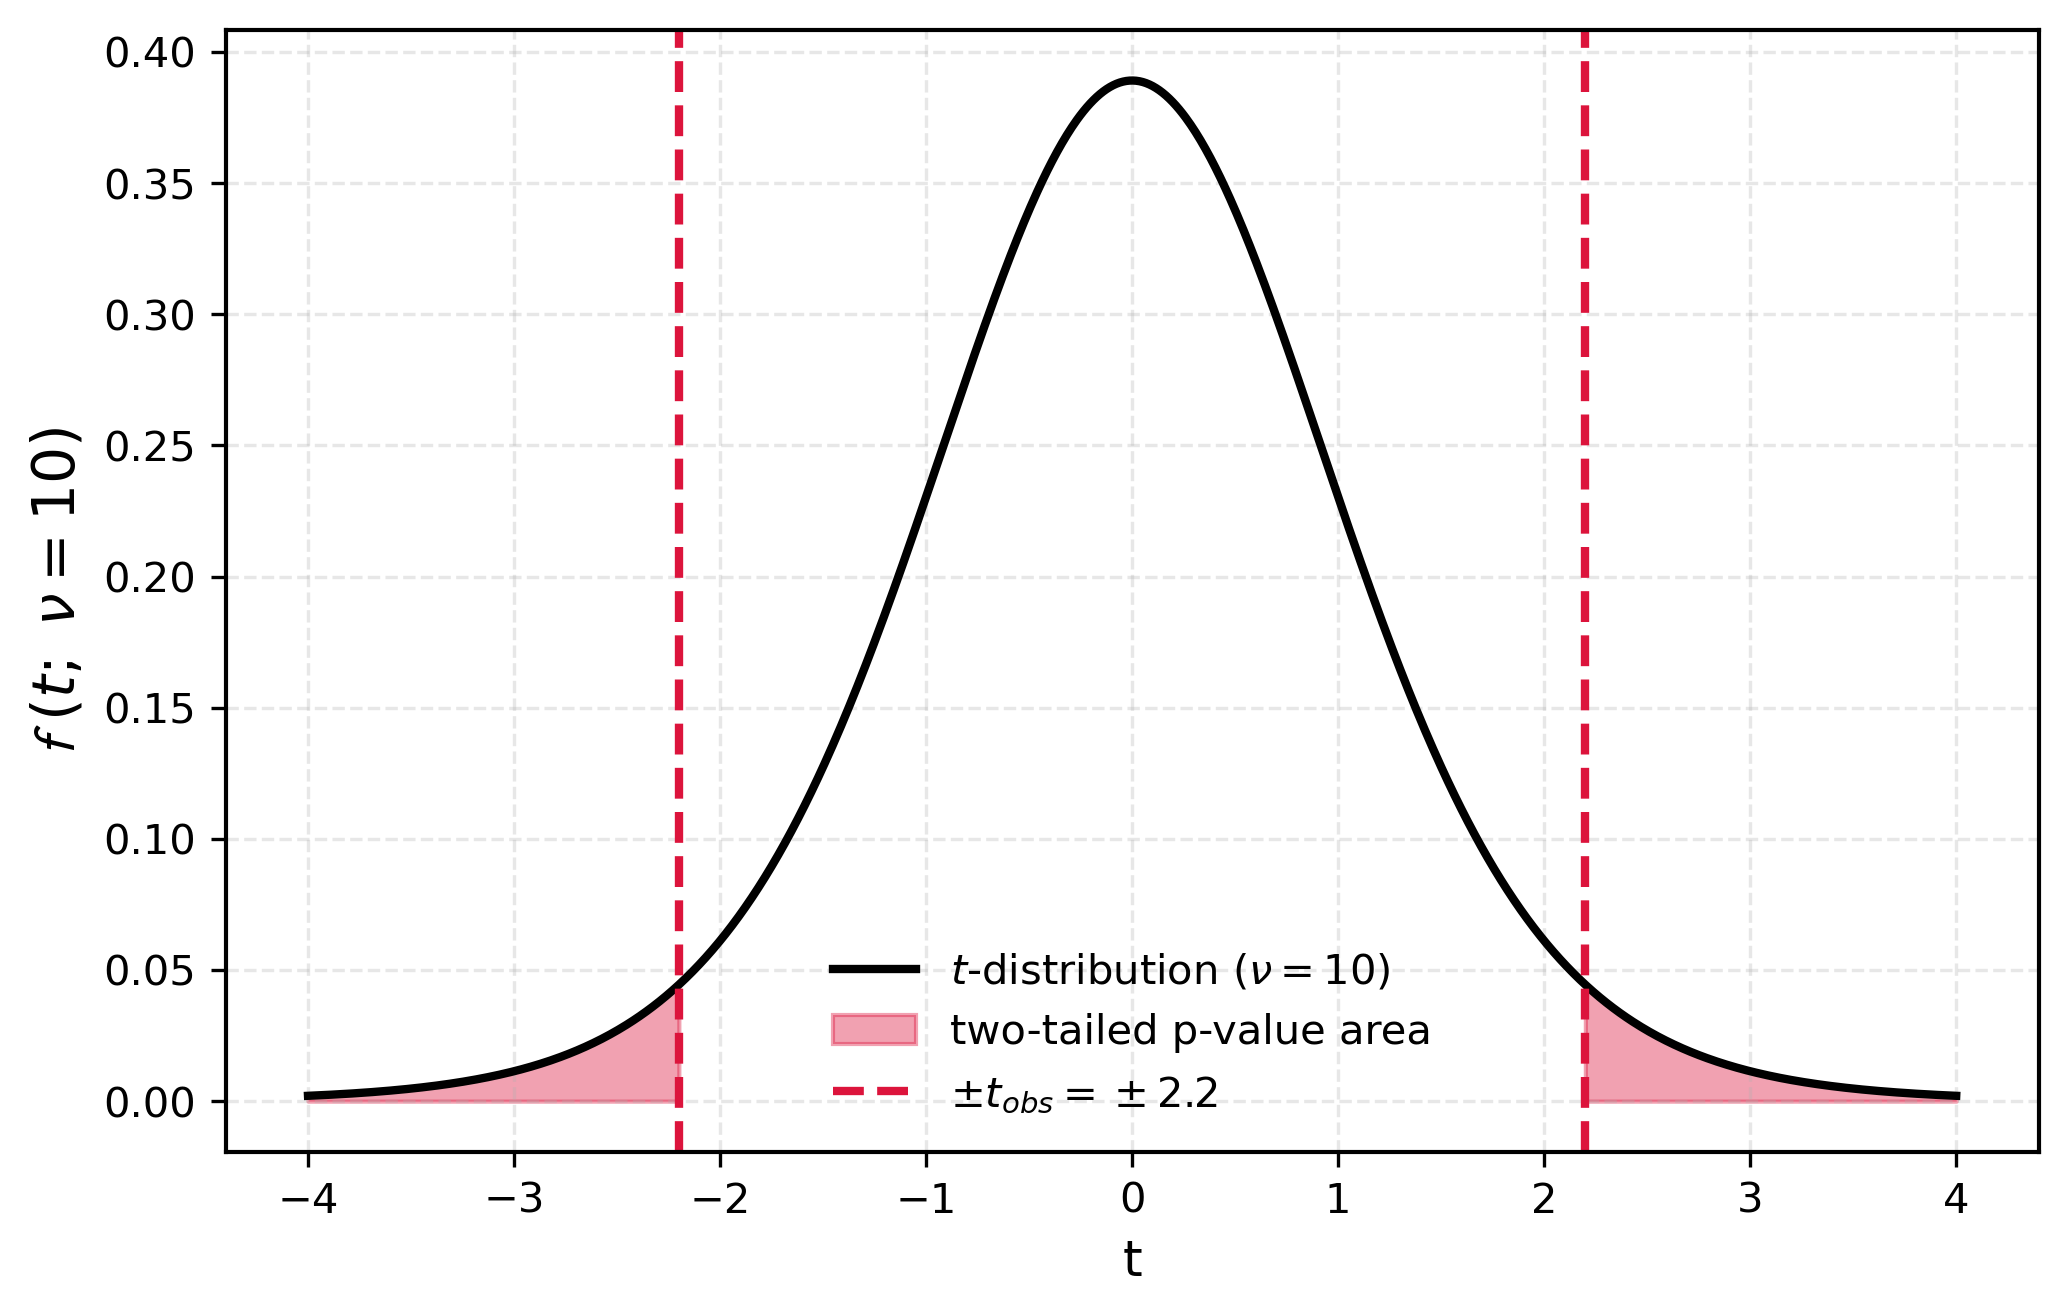
\includegraphics[width=0.7\textwidth]{figures/chapter4/t_test_1_sample_p_two_tailed.png}
    \caption{Representation of the t statistic, following the Student's t distribution, for a particular value of the degrees of freedom ($\nu = 10$). The integral of the shadowed area represents the \textit{2-sided}, or \textit{2-tailed} p-value, as the probability of obtaining a result \textit{at least as extreme} as the one obtained $t_{obs}$.}
    \label{fig:t_test2}
\end{figure}

The next example we will encounter is an extension of the same question. The so-called \textit{two-sample t-test} is used to determine whether the sample means of two sets of observations are significantly different from one another. It assumes that the sample data are drawn from a normally distributed population. The test statistic is given by:
\[
    t = \frac{\bar{x}_{1} - \bar{x}_{2}}{\sqrt{\big(n_{1} - 1)^{2} + (n_{2} - 1)^{2}}},
\]
where $\bar{x}$ is the sample mean, $\mu$ is the population mean, $s$ is the sample standard deviation, and $n$ is the sample size.\\

The computation of the p-value:
\[
p = P\left(t > t obs \right) = 2 \cdot \int_{|t|}^{\infty} f_{T_{df}}(x)\,dx = 2 \cdot \left[1 - F_{T_{df}}(|t|)\right]
\]

Being $f_{T_{n-1}}$ the PDF of the t variable, the \textit{Student's t distribution} with $n_1 + n_2 - 1$ degrees of freedom, and $F_{T_{n-1}}$ the corresponding cumulative distribution
Note here we assume equal variances. For Welch’s t-test (unequal variances), use the same form, but with Welch-adjusted [...]

\subsection*{The t distribution}

For two independent samples \( X_1, \ldots, X_n \sim \mathcal{N}(\mu_1, \sigma^2) \) and \( Y_1, \ldots, Y_m \sim \mathcal{N}(\mu_2, \sigma^2) \), the test statistic is:
\[
t = \frac{\bar{X} - \bar{Y}}{S_p \sqrt{\frac{1}{n} + \frac{1}{m}}}
\]
with pooled variance estimate:
\[
S_p^2 = \frac{(n-1)S_X^2 + (m-1)S_Y^2}{n + m - 2}
\]

Under \( H_0: \mu_1 = \mu_2 \), the statistic follows a \textit{t}-distribution with \( n + m - 2 \) degrees of freedom:
\[
t \sim t_{n+m-2}
\]
Distribution and computation of the p-value as defined above.

\begin{figure}[ht]
    \centering
    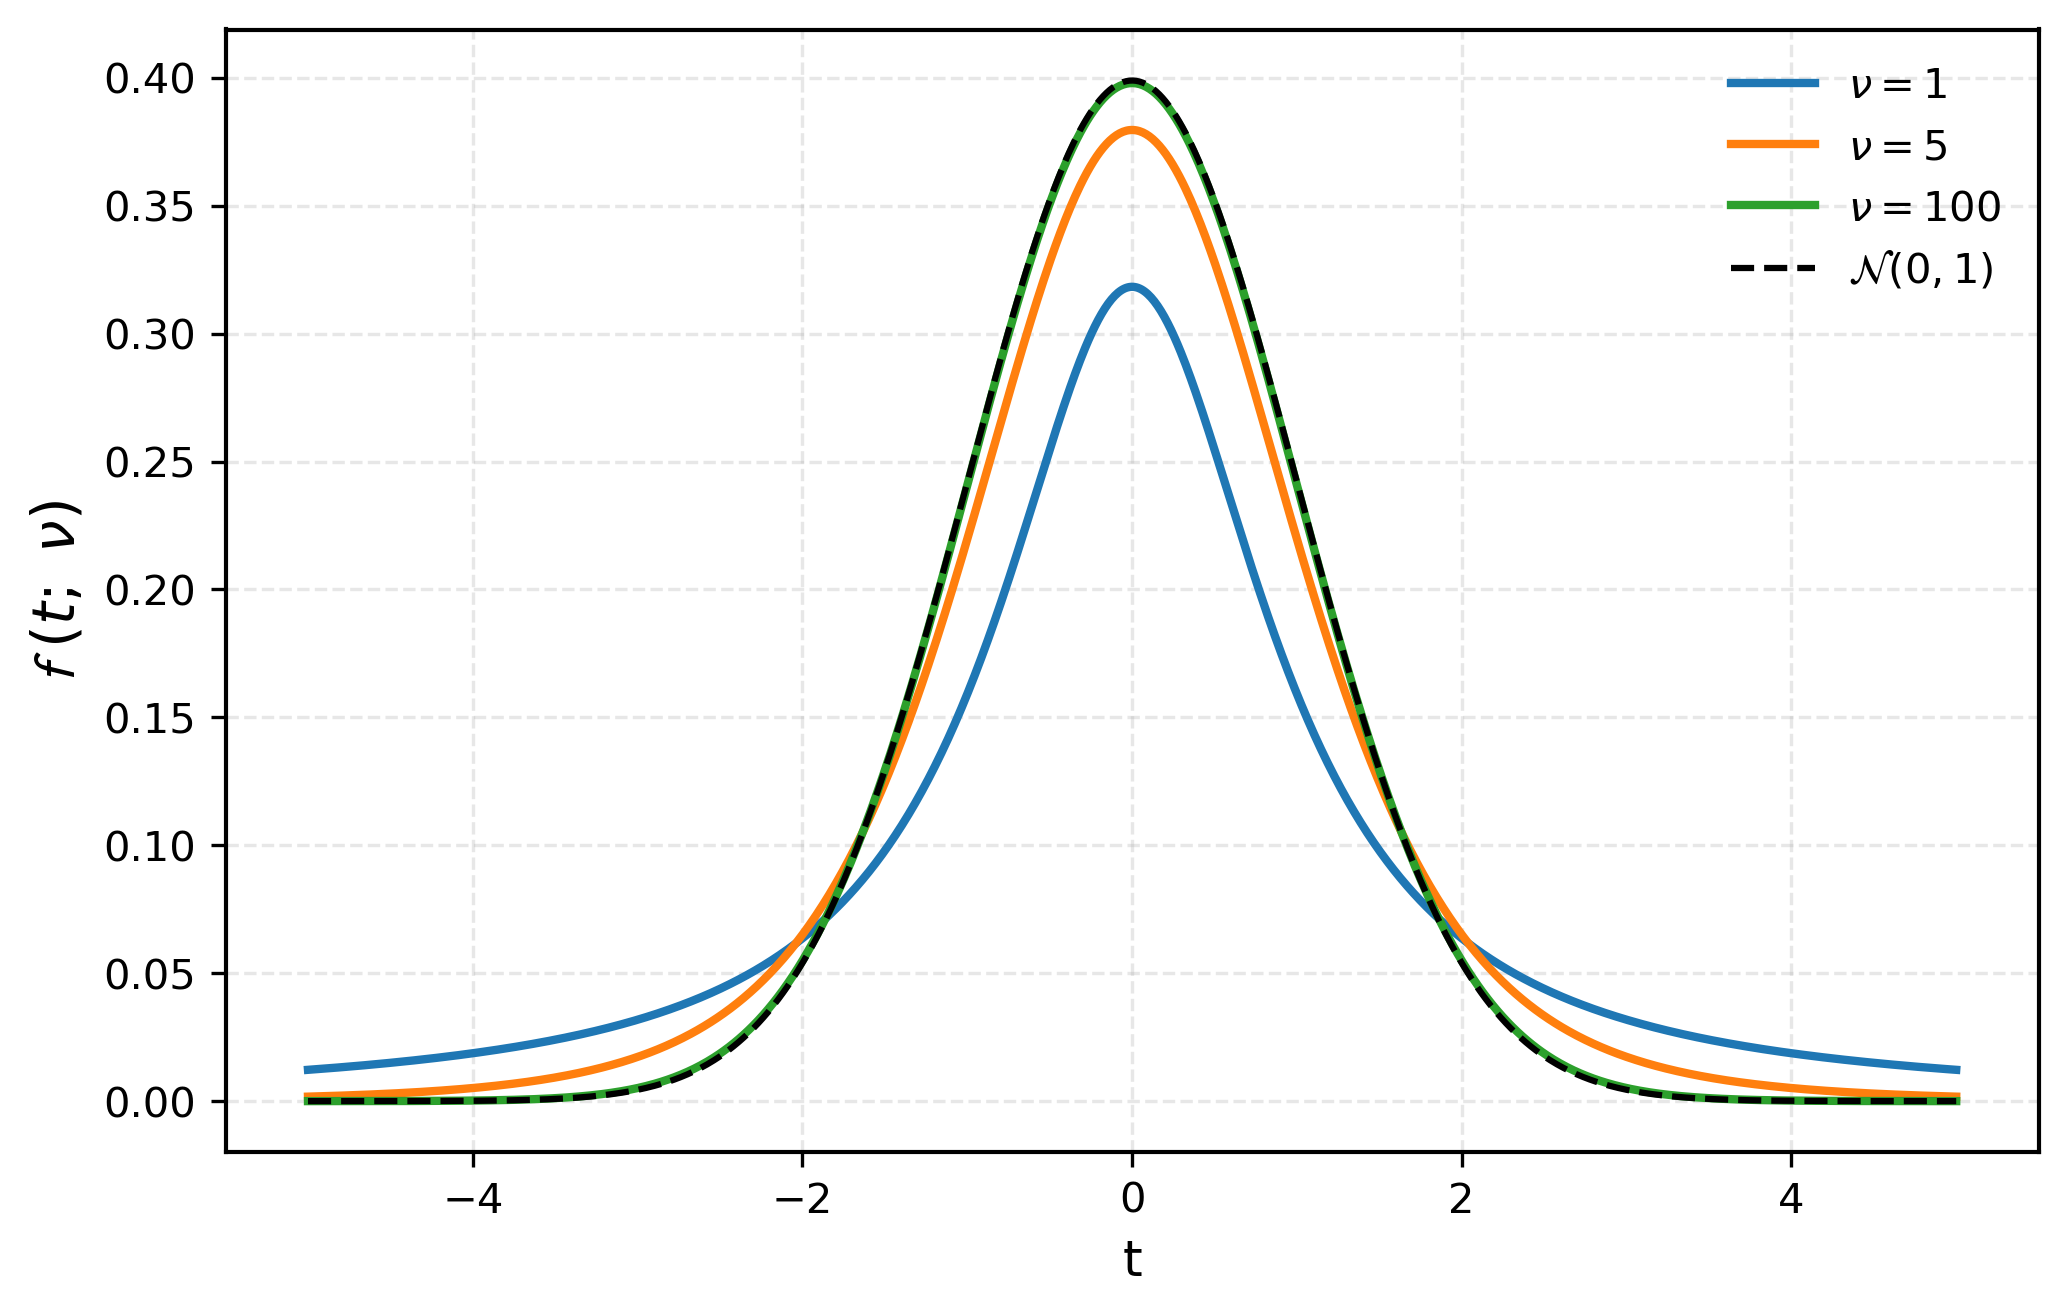
\includegraphics[width=0.7\textwidth]{figures/chapter4/t_distribution.png}
    \caption{Representation of the Student's t distribution, for different values of the degrees of freedom $\nu$.}
    \label{fig:t_distribution}
\end{figure}

\newpage

\subsection{Compare sample variances of two groups - Fisher's exact test}

Fisher’s exact test, introduced by Ronald A. Fisher in the 1930s, occupies a unique place in the statistical repertoire as a method built not on approximation, but on exact combinatorial reasoning. Designed to test for nonrandom association between two categorical variables in a 2x2 contingency table, the test calculates the exact probability of obtaining the observed configuration—or one more extreme—under the null hypothesis of independence. Unlike the chi-squared test, which relies on asymptotic assumptions, Fisher’s exact test makes no concession to large-sample theory, rendering it particularly well-suited for small datasets where expected counts may be sparse \cite{welch1947}.\\

The genesis of the test is as intellectual as it is practical. Fisher, with his characteristic synthesis of biological intuition and statistical rigor, crafted the test to address problems in genetics and experimental design. In particular, he sought a method that preserved the integrity of inference even when data were limited—a not uncommon situation in biological sciences of his time. His test exemplifies his broader philosophical stance: that statistical methods should be exact, and that inferences should reflect the full structure of the data, not rely on approximations that may distort conclusions.\\

In modern usage, Fisher’s exact test continues to shine in small-sample contexts—such as clinical trials, epidemiology, and case-control studies—where cell counts are low and the cost of misjudging association is high. Its continued relevance, despite the availability of powerful computational tools and large datasets, underscores a broader truth: that precision in reasoning often matters as much as the scale of inquiry. The test embodies an ideal of statistical craftsmanship, where fidelity to the data is preserved down to the last permutation.\\

\begin{figure}[ht]
    \centering
    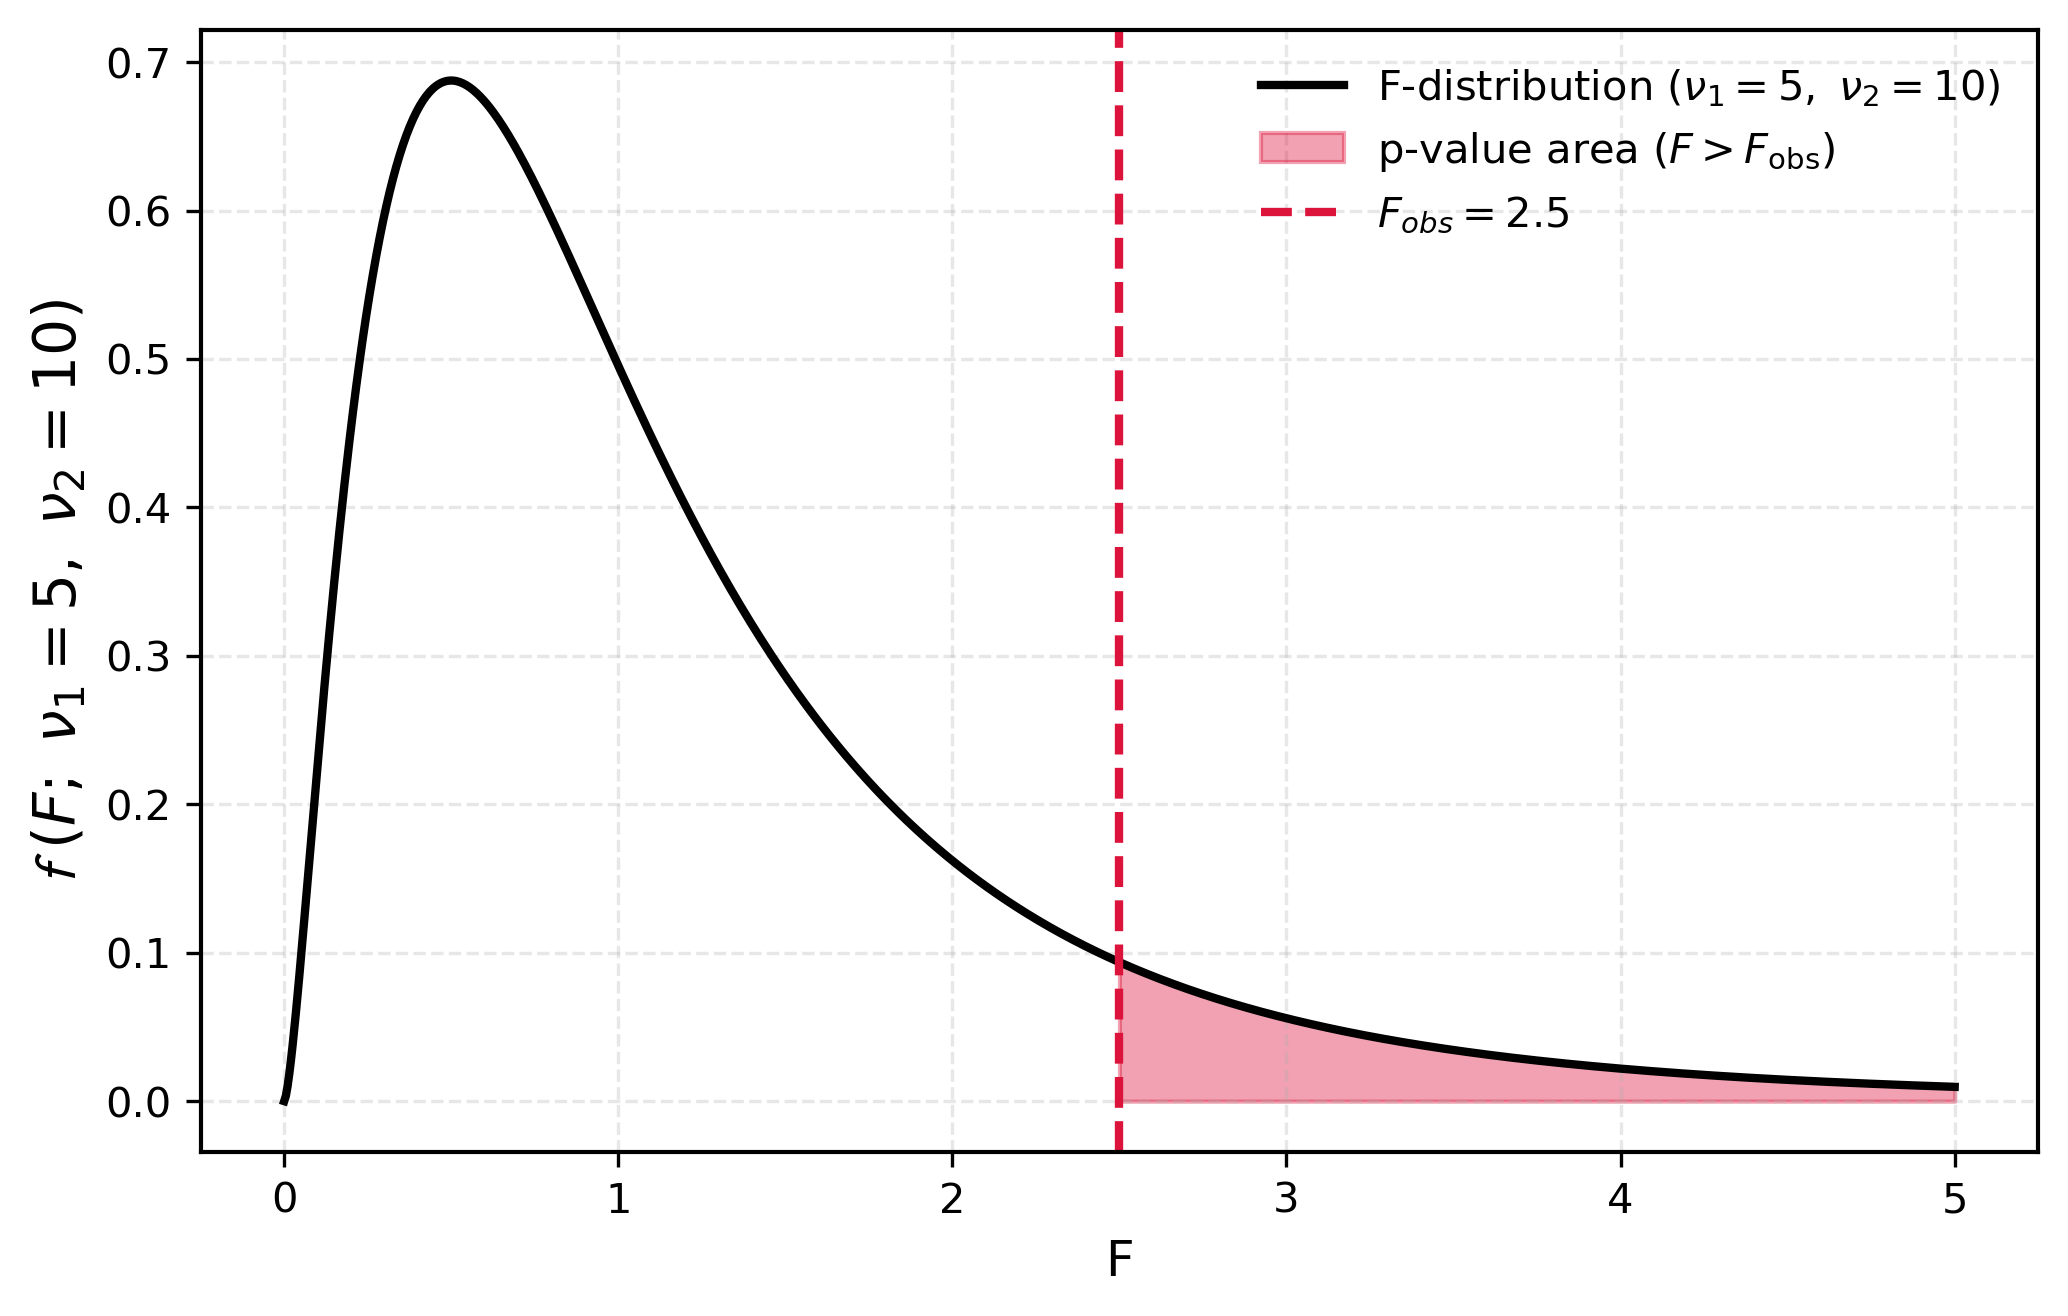
\includegraphics[width=0.7\textwidth]{figures/chapter4/f_test_one_tailed.png}
    \caption{Representation of the F statistic, following the Fisher distribution, for a particular value of the degrees of freedom ($\nu = 10$). The integral of the shadowed area represents the \textit{1-sided}, or \textit{1-tailed} p-value, as the probability of obtaining a result \textit{at least as extreme} as the one obtained $t_{obs}$.}
    \label{fig:f_test1}
\end{figure}

The next example we will encounter is an extension of the same question., The so-called \textit{Fisher t-test}, or just $F$ test, is used to determine whether the sample variances of two sets of observations are significantly different from one another. It assumes that the sample data are drawn from a normally distributed population.\\

The F statistic is a ratio of two independent variance estimates, each scaled by their respective degrees of freedom. It is used to test whether group variances (or group means, in ANOVA) differ significantly. The general form of the F statistic is:
\[
F = \frac{S_1^2 / \nu_1}{S_2^2 / \nu_2}
\]

where $s_1^{2}$ and $s_2^{2}$ are the sample variances, and the degrees of freedom are $d_1 = n_1 - 1$ and $d_2 = n_2 - 1$.\\

The computation of the p-value:
\[
p = \sum_{\text{extreme values}} \frac{\binom{a+b}{a} \binom{c+d}{c}}{\binom{n}{a+c}}
\]

Under the null hypothesis, the F statistic follows the F-distribution:

\[
F \sim F(\nu_1, \nu_2)
\]

and the p-value is computed as the upper-tail probability:

\[
p = P(F_{\nu_1, \nu_2} \geq F_{\text{obs}}) = \int_{F_{\text{obs}}}^{\infty} f_{F_{\nu_1, \nu_2}}(x)\,dx
\]

\subsection*{The F distribution}

When the assumption of equal variances is violated, the test statistic is:
\[
t = \frac{\bar{X} - \bar{Y}}{\sqrt{\frac{S_X^2}{n} + \frac{S_Y^2}{m}}}
\]
with an approximate degrees of freedom:
\[
\nu \approx \frac{\left(\frac{S_X^2}{n} + \frac{S_Y^2}{m}\right)^2}{\frac{(S_X^2/n)^2}{n - 1} + \frac{(S_Y^2/m)^2}{m - 1}}
\]

Under the null \( H_0: \mu_1 = \mu_2 \), the distribution of \( t \) is approximated by:
\[
t \sim t_{\nu}
\]
Distribution and computation of the p-value as defined above.

\newpage

\subsection{Compare variation on more than two groups - Fisher's ANOVA}

The analysis of variance, or ANOVA, is one of the 20th century's major statistical innovations, largely credited to Ronald Fisher, who formalized it in the 1920s while working at the Rothamsted Experimental Station. Its core purpose is to partition total variation in a dataset into components attributable to different sources—typically, between-group variation and within-group (error) variation. ANOVA provides a systematic method for comparing more than two means simultaneously, resolving what would otherwise require a series of pairwise t tests and an increasing risk of Type I error 
\cite{fisher1925}.\\

Conceptually, ANOVA represents a unifying idea: that observed data contain structure and randomness, and that the task of statistical inference is to disentangle them. It was particularly well-suited to agricultural experiments, where multiple treatments were applied across randomized plots, and variation needed to be measured with mathematical elegance and practical clarity. Fisher’s framework gave researchers a way to understand experimental results in terms of their statistical "signal," paving the way for rigorous design and interpretation across many scientific disciplines.\\

Today, ANOVA remains foundational in experimental science, psychology, and the social sciences. Its principles have expanded into more complex models—repeated measures, factorial designs, and mixed effects frameworks—but the essential logic endures. It is a statistical lens through which variability is not merely noise, but an object of structured inquiry. In this way, ANOVA reflects a deeper epistemological commitment: that difference can be measured, that structure can be inferred, and that complexity, when properly modeled, reveals its underlying form.\\

\begin{figure}[ht]
    \centering
    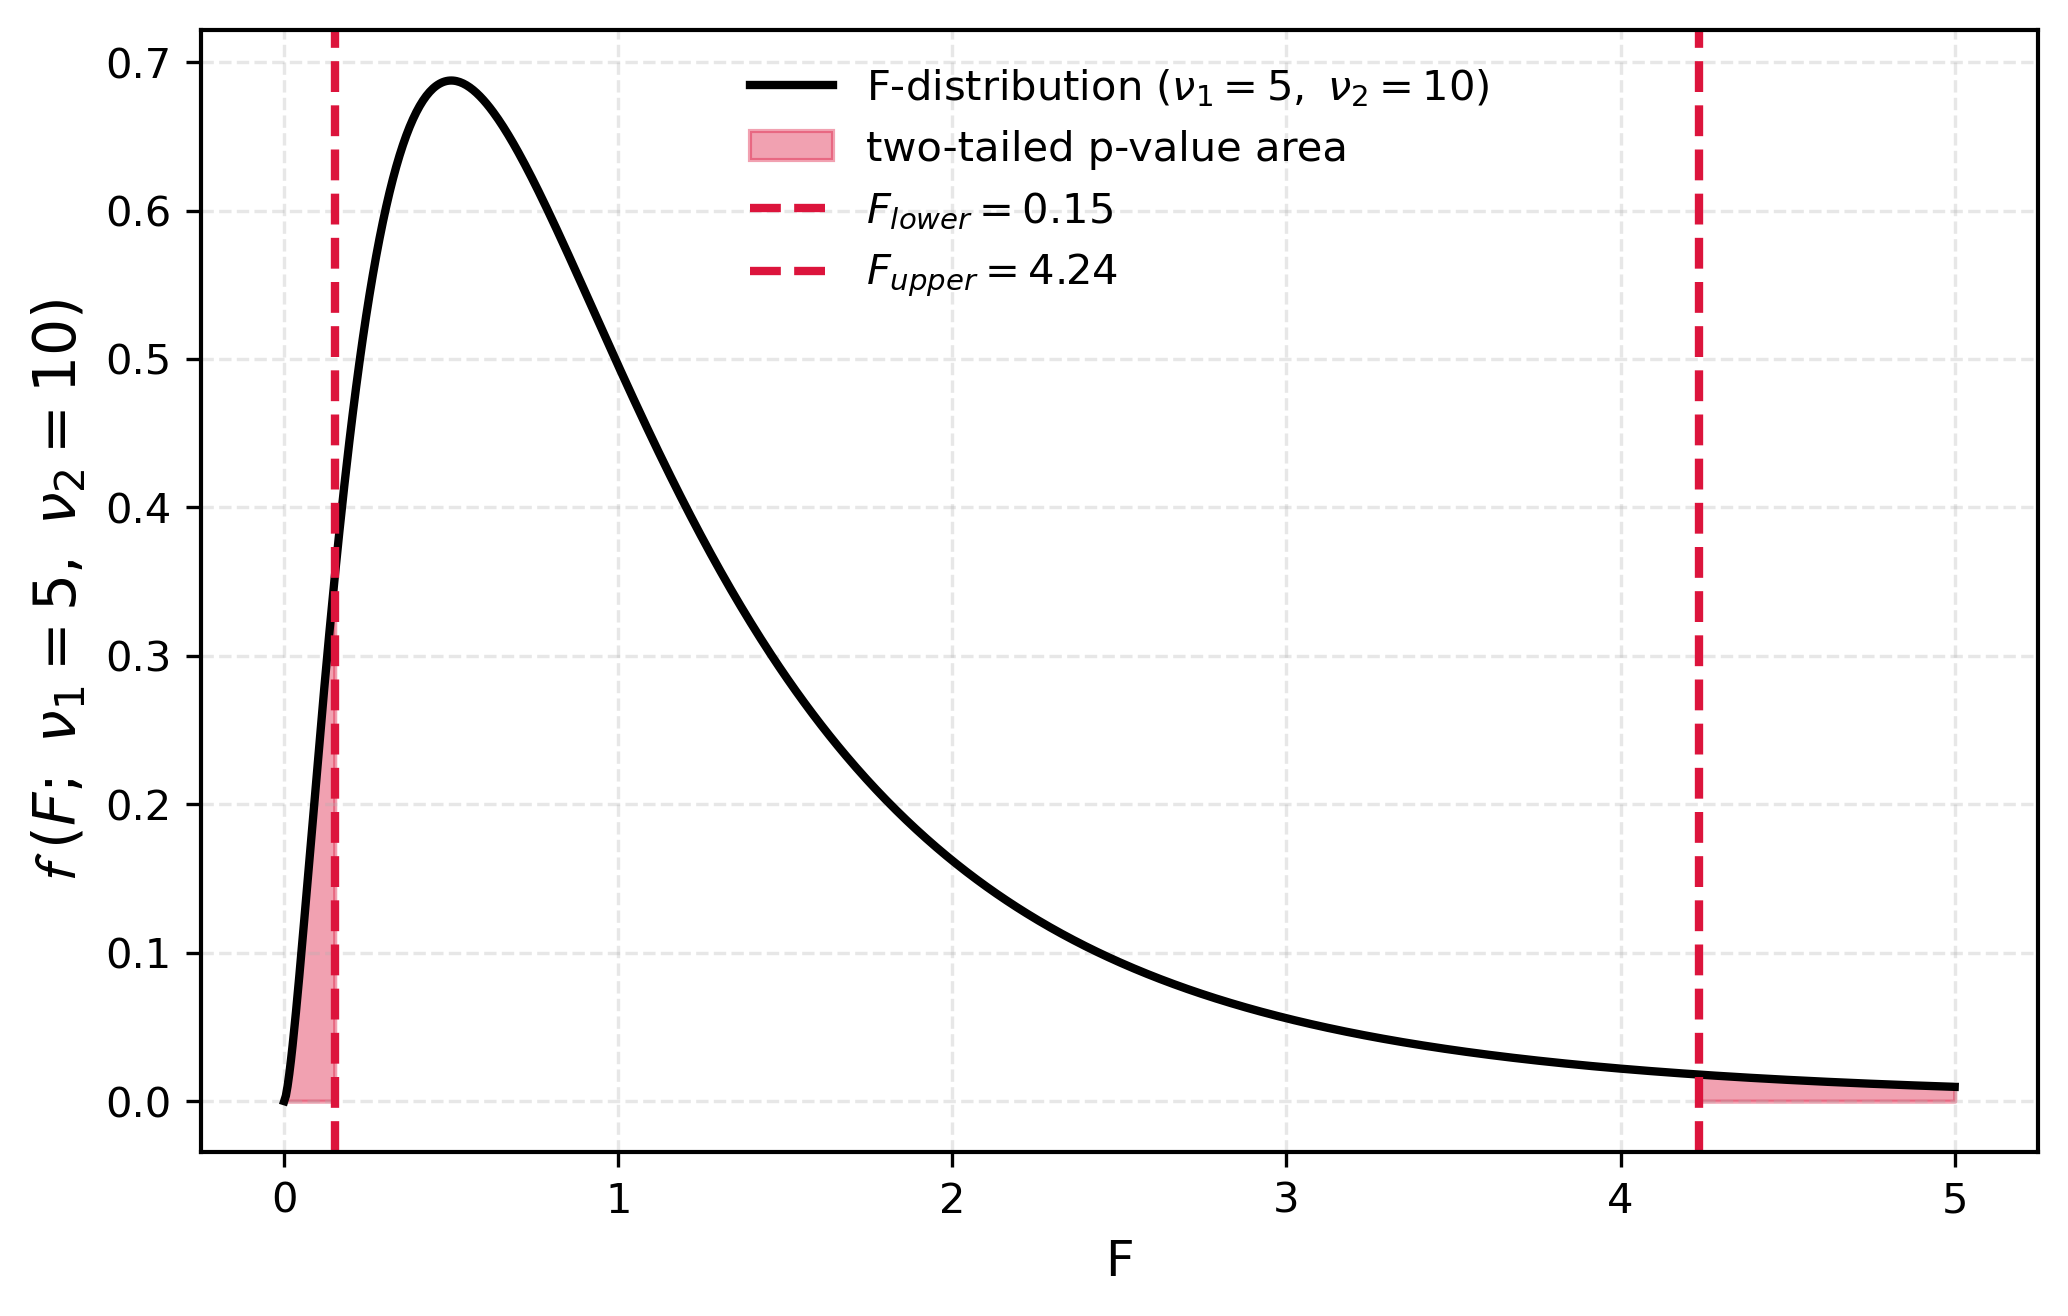
\includegraphics[width=0.7\textwidth]{figures/chapter4/f_test_two_tailed.png}
    \caption{Representation of the F statistic, following the Fisher distribution, for a particular value of the degrees of freedom ($\nu = 10$). The integral of the shadowed area represents the \textit{2-sided}, or \textit{2-tailed} p-value, as the probability of obtaining a result \textit{at least as extreme} as the one obtained $t_{obs}$.}
    \label{fig:f_test2}
\end{figure}

The so-called Analysis of Variance, one way ANOVA, or just ANOVA, is used to determine whether the variation of a dataset comes primary from variation within the samples themselves, or from variation between the groups. It is an extension of the Fisher test, where the F statistic is computed as:
\[
    f(x; d_{1}, d_{2}) = \frac{s_\text{between}^{2}}{s_\text{within}^{2}},
\]
where $s_1^{2}$ and $s_2^{2}$ are the sample variances, and the degrees of freedom are $d_1 = n_1 - 1$ and $d_2 = n_2 - 1$.\\

\[
F = \frac{MS_{\text{between}}}{MS_{\text{within}}} = \frac{SS_{\text{between}} / (k - 1)}{SS_{\text{within}} / (N - k)}
\]

where:
\begin{itemize}
  \item $SS_{\text{between}}$ is the sum of squares between groups,
  \item $SS_{\text{within}}$ is the sum of squares within groups,
  \item $k$ is the number of groups,
  \item $N$ is the total number of observations.
\end{itemize}

The computation of the p-value:
\[
p = \int_{F}^{\infty} f_{F_{df_1, df_2}}(x)\,dx = 1 - F_{F_{df_1, df_2}}(F)
\]

\subsection*{The F distribution}

Assume \( k \) groups with sample sizes \( n_i \) and group means \( \bar{X}_i \). The test statistic is:
\[
F = \frac{MS_{\text{between}}}{MS_{\text{within}}} = \frac{SS_{\text{between}} / (k - 1)}{SS_{\text{within}} / (N - k)}
\]
with:
\[
SS_{\text{between}} = \sum_{i=1}^{k} n_i (\bar{X}_i - \bar{X})^2, \quad SS_{\text{within}} = \sum_{i=1}^{k} \sum_{j=1}^{n_i} (X_{ij} - \bar{X}_i)^2
\]

Under \( H_0: \mu_1 = \mu_2 = \cdots = \mu_k \), the statistic follows:
\[
F \sim \mathcal{F}_{k-1, N-k}
\]
The PDF of the \( \mathcal{F}_{d_1, d_2} \) distribution is:
\[
f(x) = \frac{1}{\mathrm{B}(d_1/2, d_2/2)} \left(\frac{d_1}{d_2}\right)^{d_1/2} \frac{x^{d_1/2 - 1}}{\left(1 + \frac{d_1}{d_2}x\right)^{(d_1 + d_2)/2}}
\]
for \( x > 0 \).

Distribution and computation of the p-value as defined above.

\begin{figure}[ht]
    \centering
    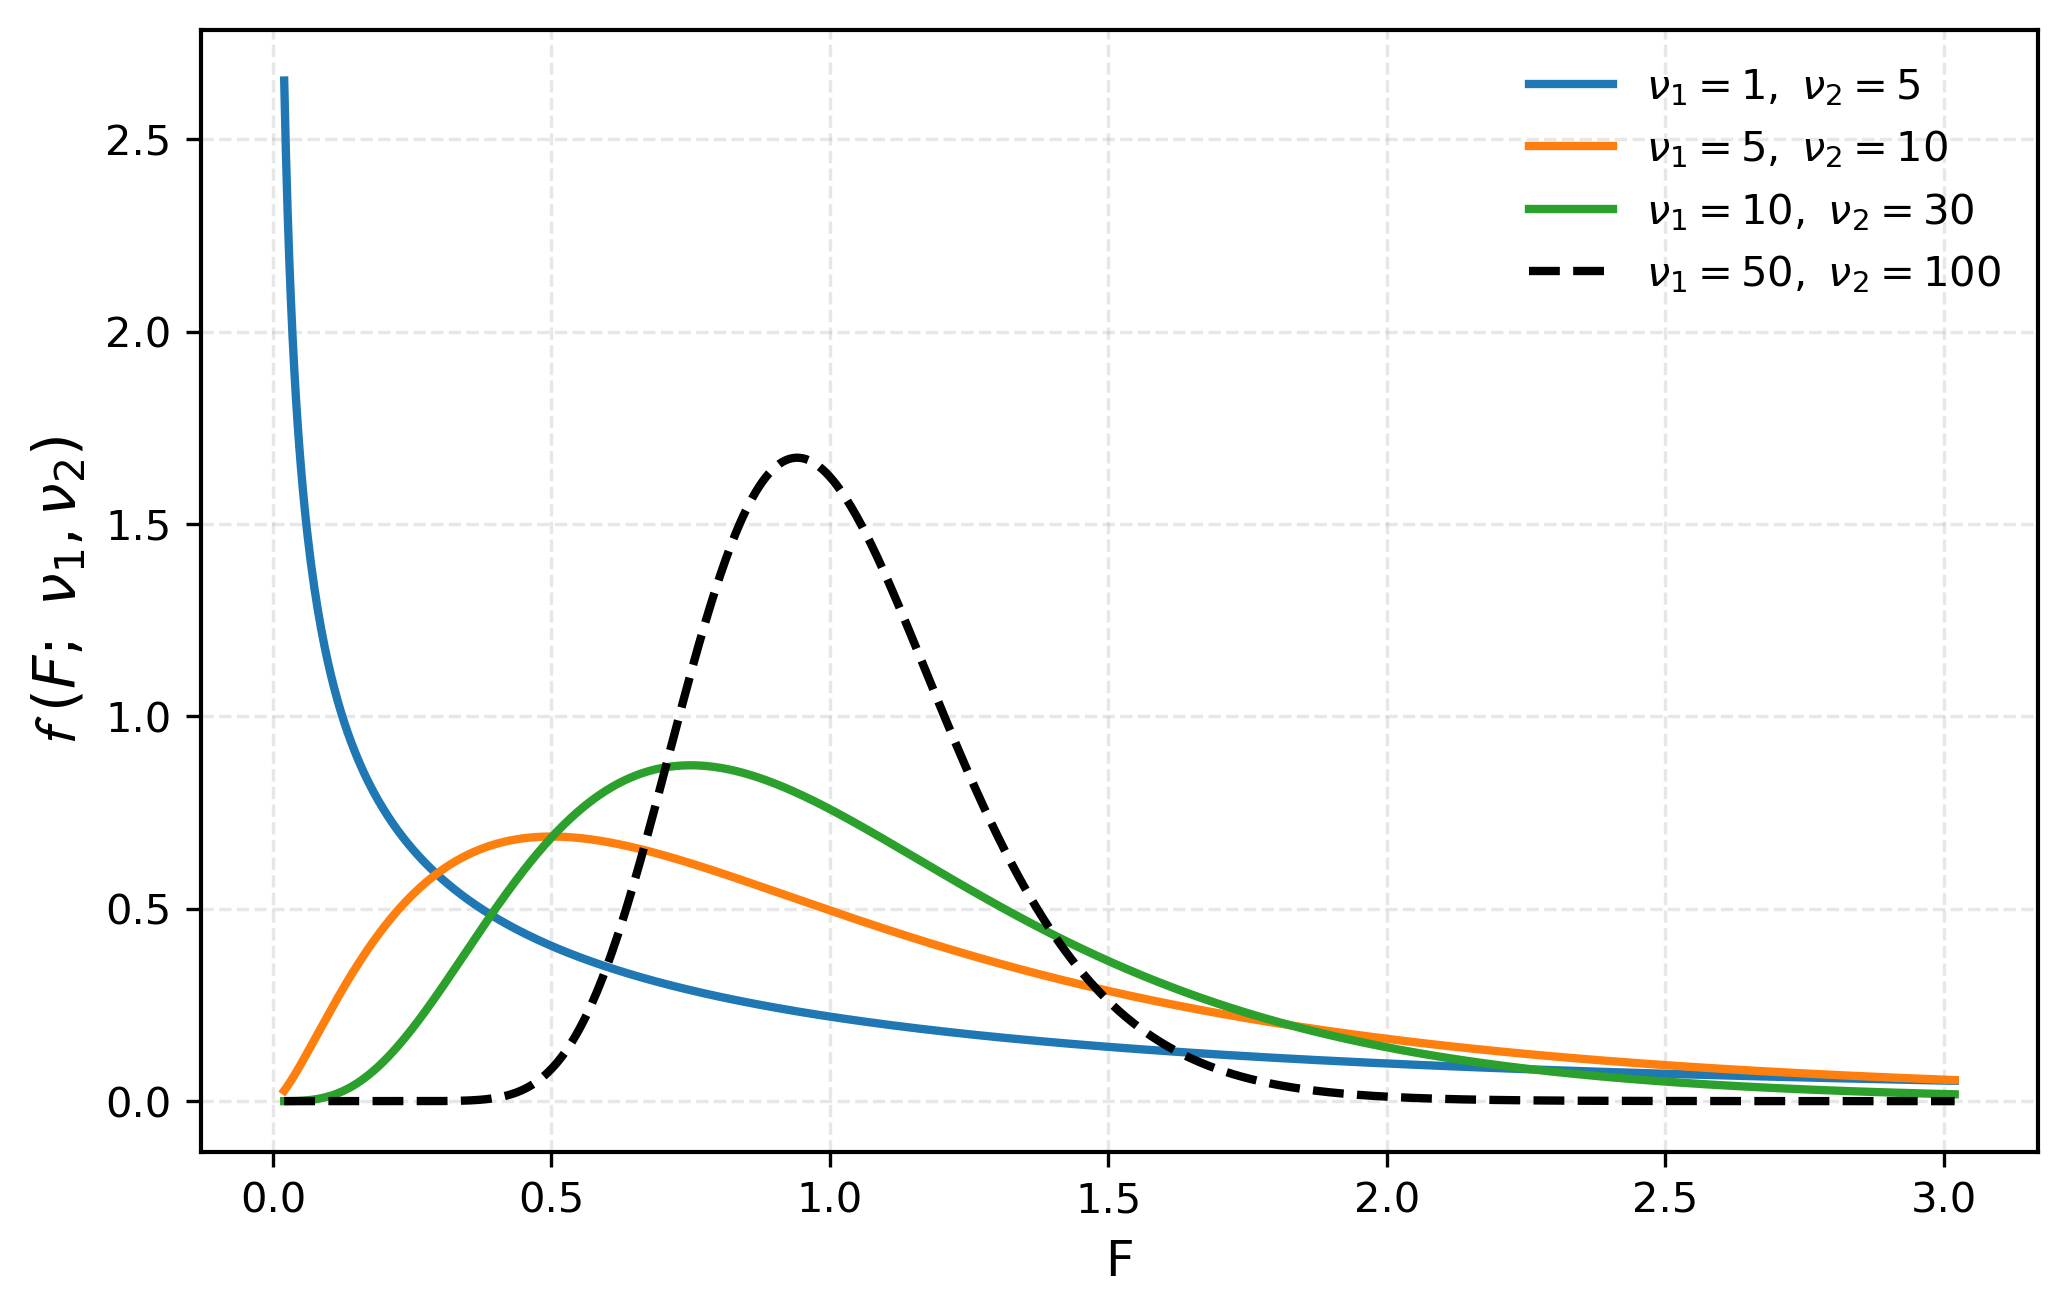
\includegraphics[width=0.7\textwidth]{figures/chapter4/f_distribution.png}
    \caption{Representation of the Fisher distribution, for different values of the degrees of freedom $\nu_1$, $\nu_2$.}
    \label{fig:f_distribution}
\end{figure}

\newpage

\subsection{Compare distributions and testing for normality - $\chi^{2}$ test}

The chi-squared test, with its roots in the work of Karl Pearson at the turn of the 20th century, stands as one of the earliest formal tests of goodness-of-fit and independence. Built on the comparison of observed frequencies to expected ones under a given hypothesis, the chi-squared statistic accumulates discrepancies between what is seen and what is statistically anticipated. It is asymptotic in nature, relying on the approximation of the chi-squared distribution, which becomes increasingly accurate with larger sample sizes and expected counts \cite{pearson1900}.\\

Pearson’s motivation was both mathematical and empirical: to provide a quantitative measure for evaluating how well a theoretical model matched observed data, particularly in biological contexts such as Mendelian genetics. His test became a cornerstone of categorical data analysis, offering a simple yet powerful method for detecting associations in contingency tables and deviations from expected distributions. Over time, the test was expanded and refined, notably by Fisher and Yates, but it has retained its essential character as a test of fit between expectation and observation.\\

In the present day, the chi-squared test continues to serve as an indispensable tool across fields as varied as market research, epidemiology, and political science. Its ability to handle complex tables and large datasets makes it well-suited to the modern data deluge. Yet its appeal also lies in its conceptual clarity: the squared discrepancy between what the world appears to be and what a hypothesis claims it should be. It is a statistical mirror, held up to the categorical world, revealing the tensions between model and reality with a cold but elegant precision.\\

\begin{figure}[ht]
    \centering
    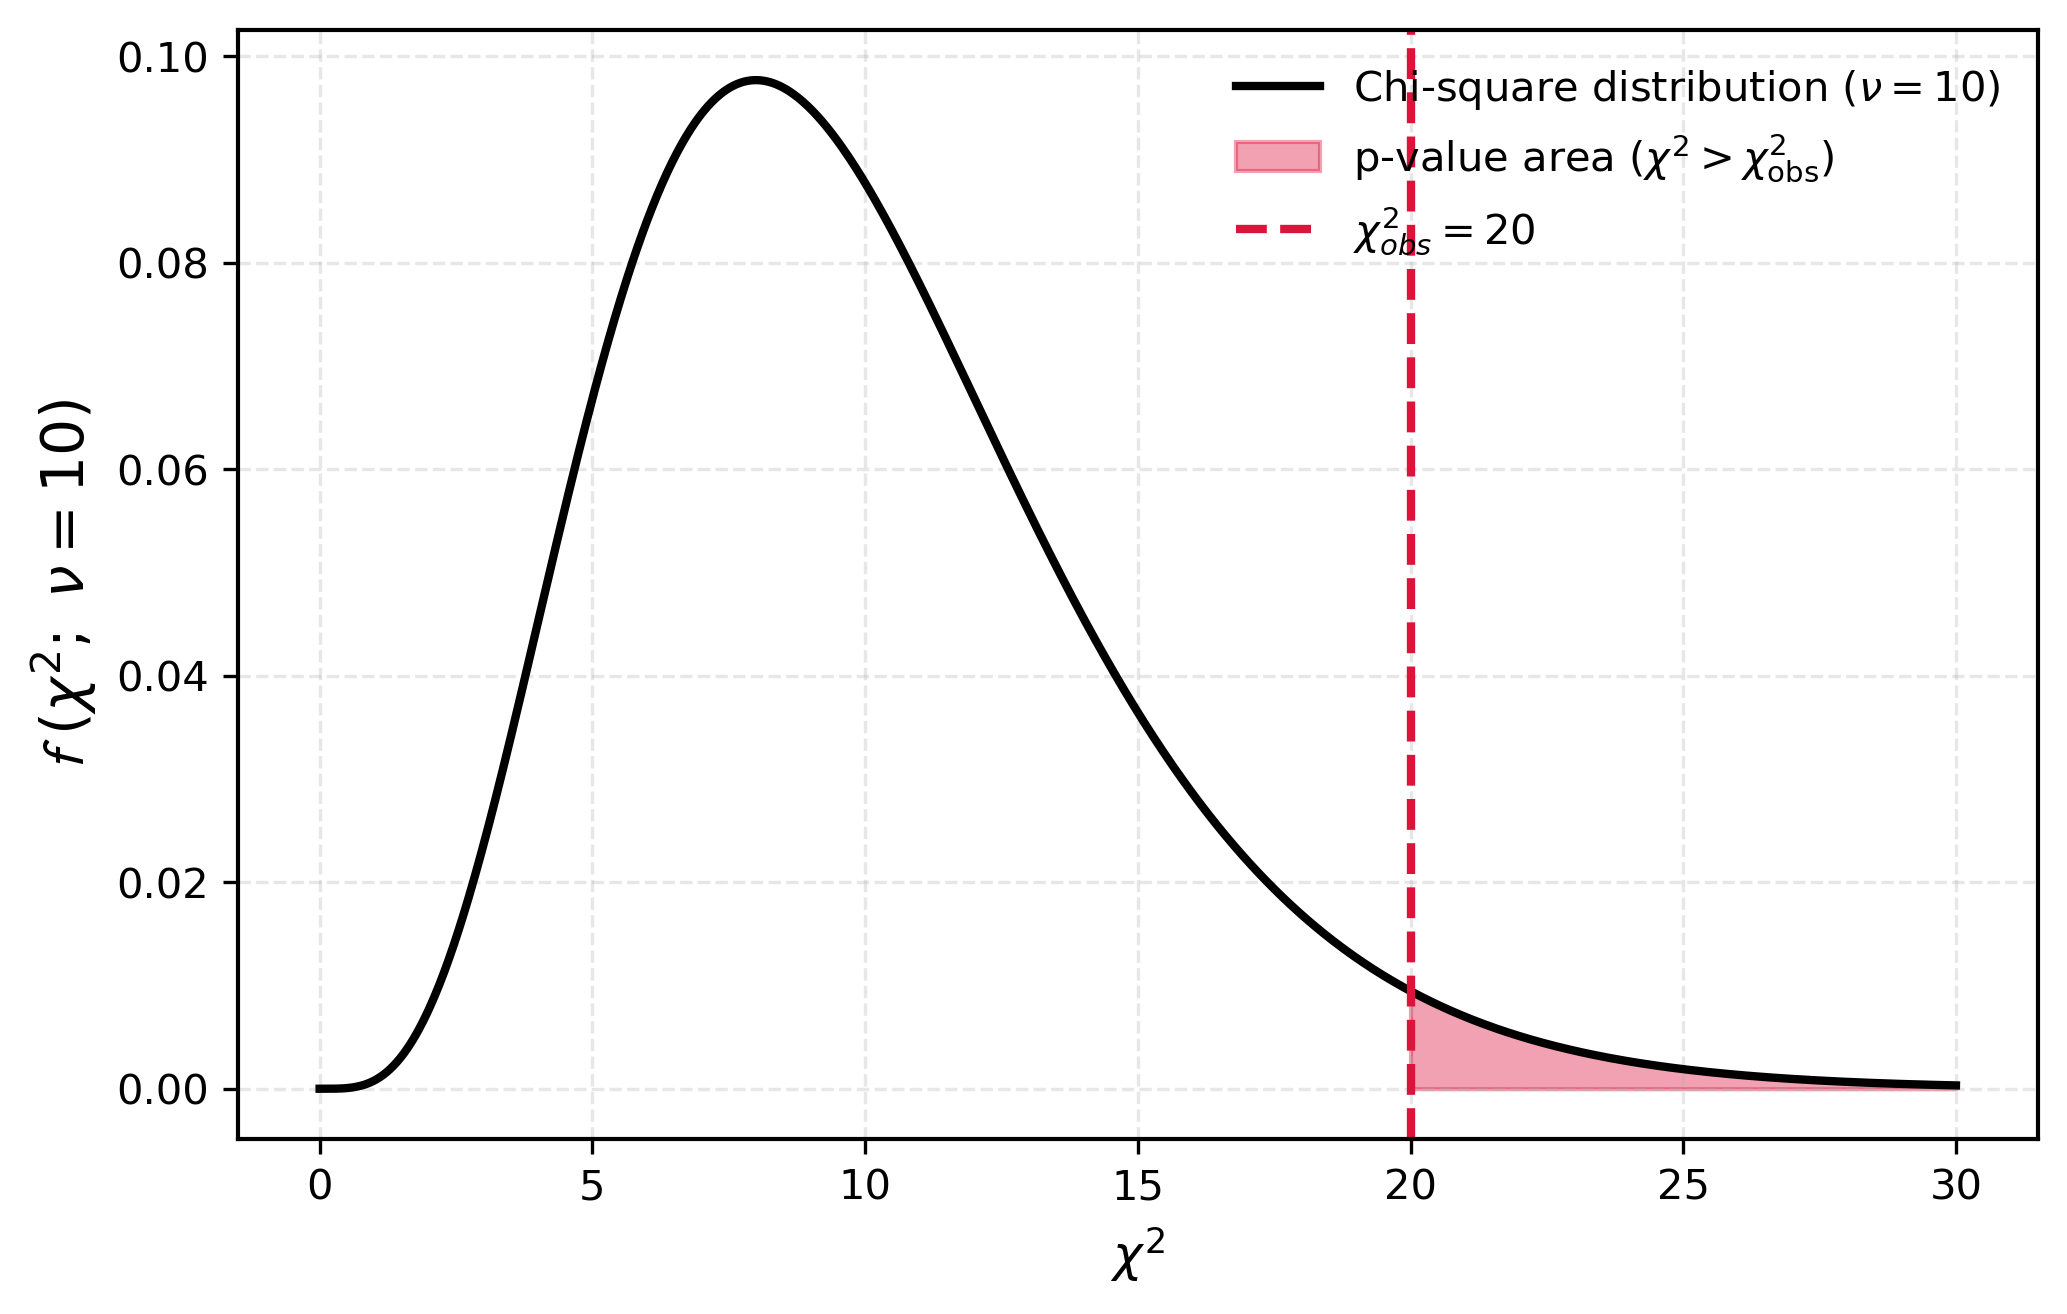
\includegraphics[width=0.7\textwidth]{figures/chapter4/chi2_test_one_tailed.png}
    \caption{Representation of the $chi^{2}$ statistic, following the Pearson $chi^{2}$ distribution, for a particular value of the degrees of freedom ($\nu = 10$). The integral of the shadowed area represents the \textit{1-sided}, or \textit{1-tailed} p-value, as the probability of obtaining a result \textit{at least as extreme} as the one obtained $chi^{2}_{obs}$.}
    \label{fig:chi2_test1}
\end{figure}

The so-called Pearson $\chi^{2}$-test is used to determine whether the set of observations is significantly different from some expected - or hypothesized - values. The $\chi^{2}$ statistic is given by:
\[
    \chi^{2}(x; N - 1) = \sum_{i = 1}^{N}\frac{(O_{i} - E{i})^{2}}{E_i},
\]
It is also used to test for normality and evaluate the goodness of a fit [...].\\\

\begin{figure}[ht]
    \centering
    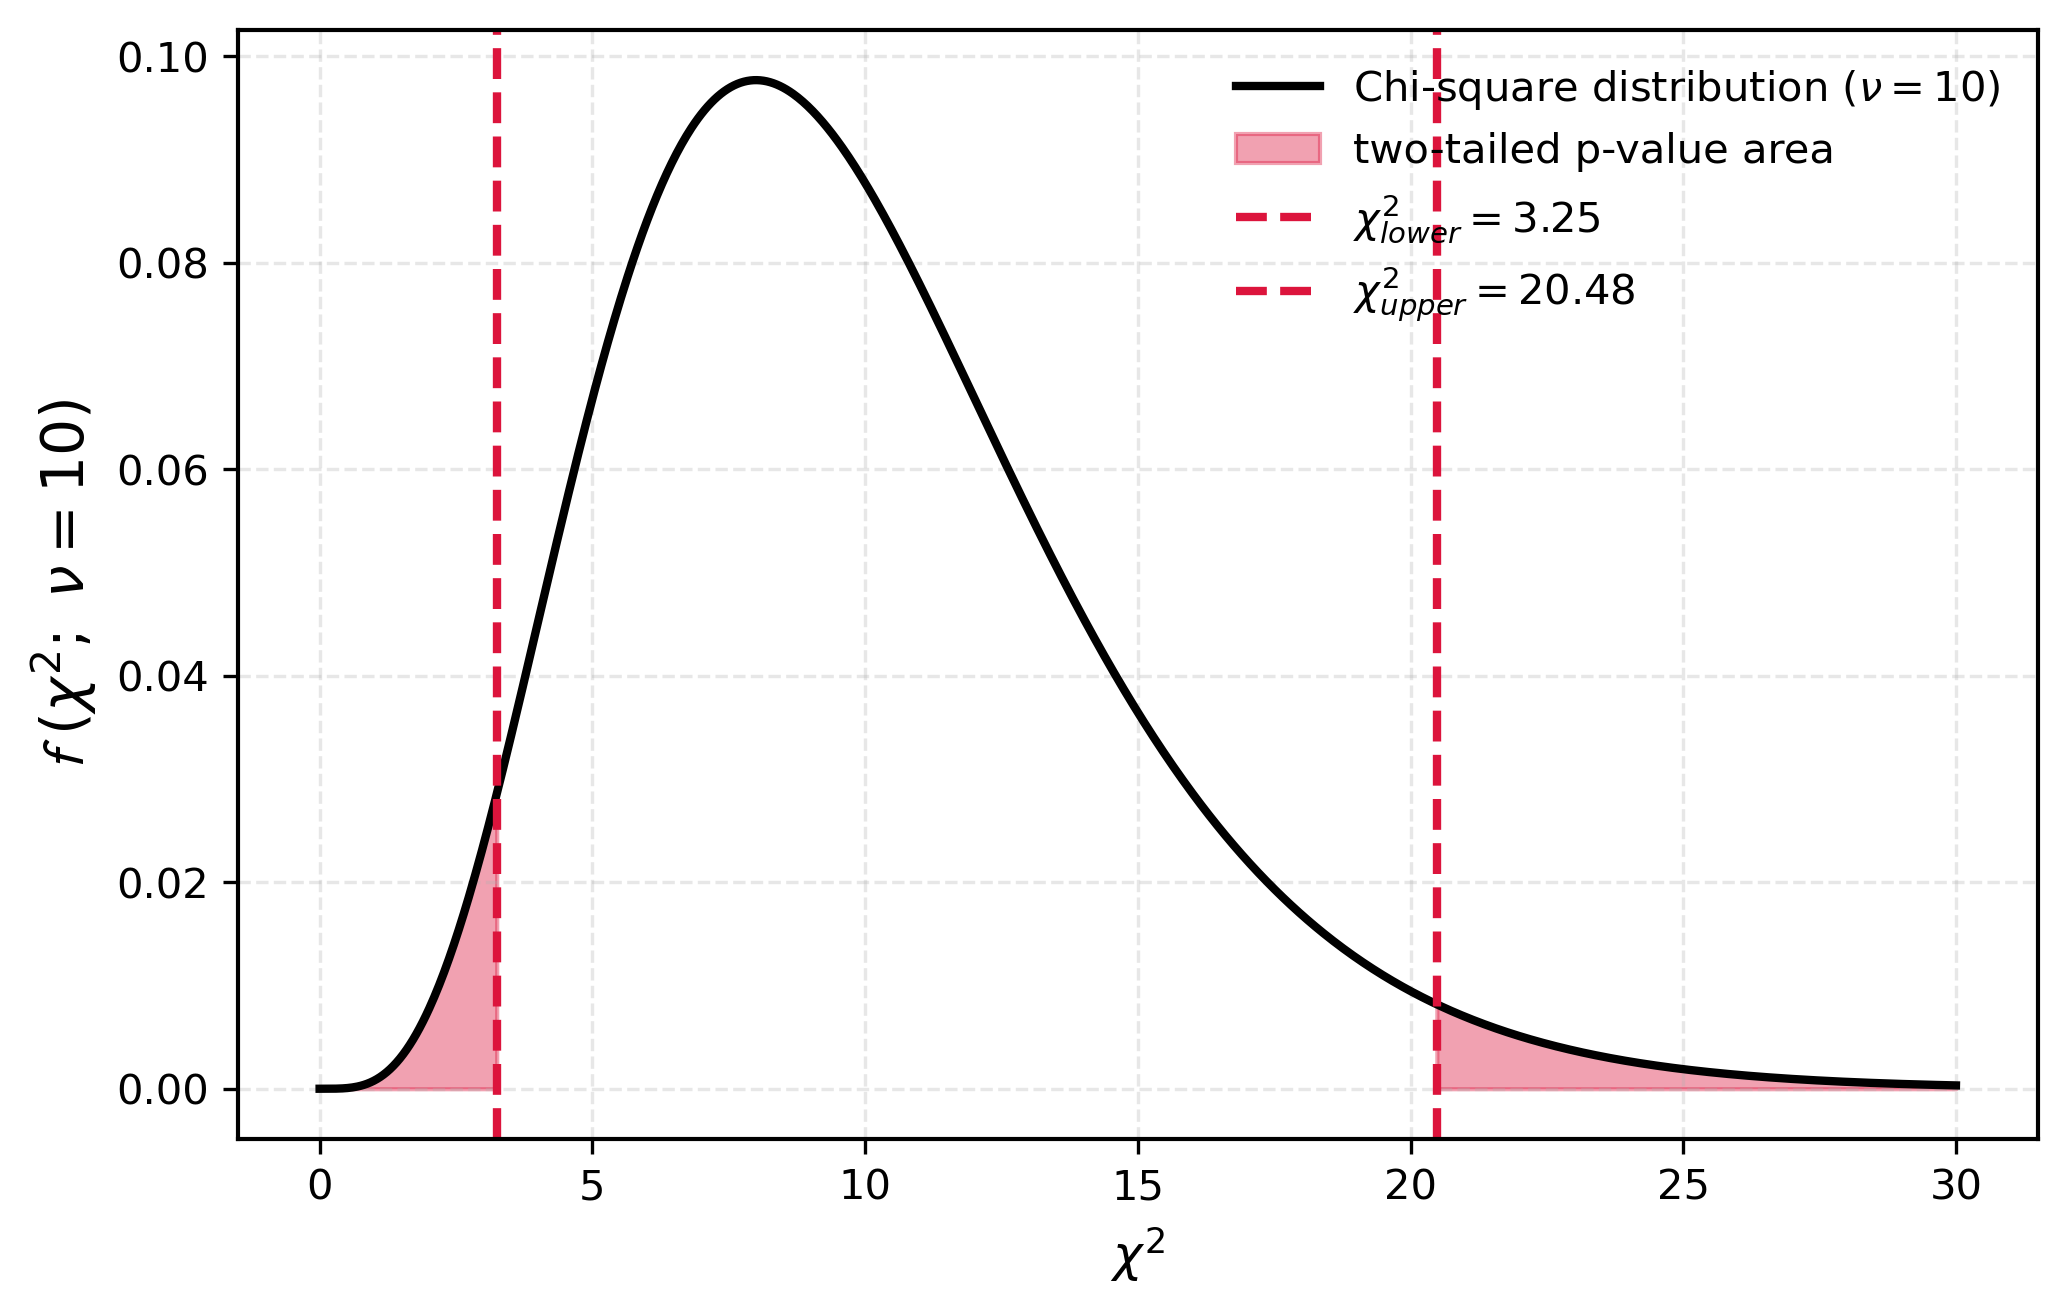
\includegraphics[width=0.7\textwidth]{figures/chapter4/chi2_test_two_tailed.png}
    \caption{Representation of the $chi^{2}$ statistic, following the Pearson $chi^{2}$ distribution, for a particular value of the degrees of freedom ($\nu = 10$). The integral of the shadowed area represents the \textit{2-sided}, or \textit{2-tailed} p-value, as the probability of obtaining a result \textit{at least as extreme} as the one obtained $chi^{2}_{obs}$.}
    \label{fig:chi2_test2}
\end{figure}

The computation of the p-value:
\[
p = \int_{\chi^2}^{\infty} f_{\chi^2_{df}}(x)\,dx = 1 - F_{\chi^2_{df}}(\chi^2)
\]

\subsection*{The $\chi^{2}$ distribution}

For observed \( O_{ij} \) and expected counts \( E_{ij} \) in an \( r \times c \) table, the test statistic is:
\[
\chi^2 = \sum_{i=1}^{r} \sum_{j=1}^{c} \frac{(O_{ij} - E_{ij})^2}{E_{ij}}
\]

Under the null hypothesis of independence, the distribution is:
\[
\chi^2 \sim \chi^2_{(r-1)(c-1)}
\]

The PDF of the chi-squared distribution with \( k \) degrees of freedom is:
\[
f(x) = \frac{1}{2^{k/2} \Gamma(k/2)} x^{k/2 - 1} e^{-x/2}, \quad x > 0
\]

Distribution and computation of the p-value as defined above.

\begin{figure}[ht]
    \centering
    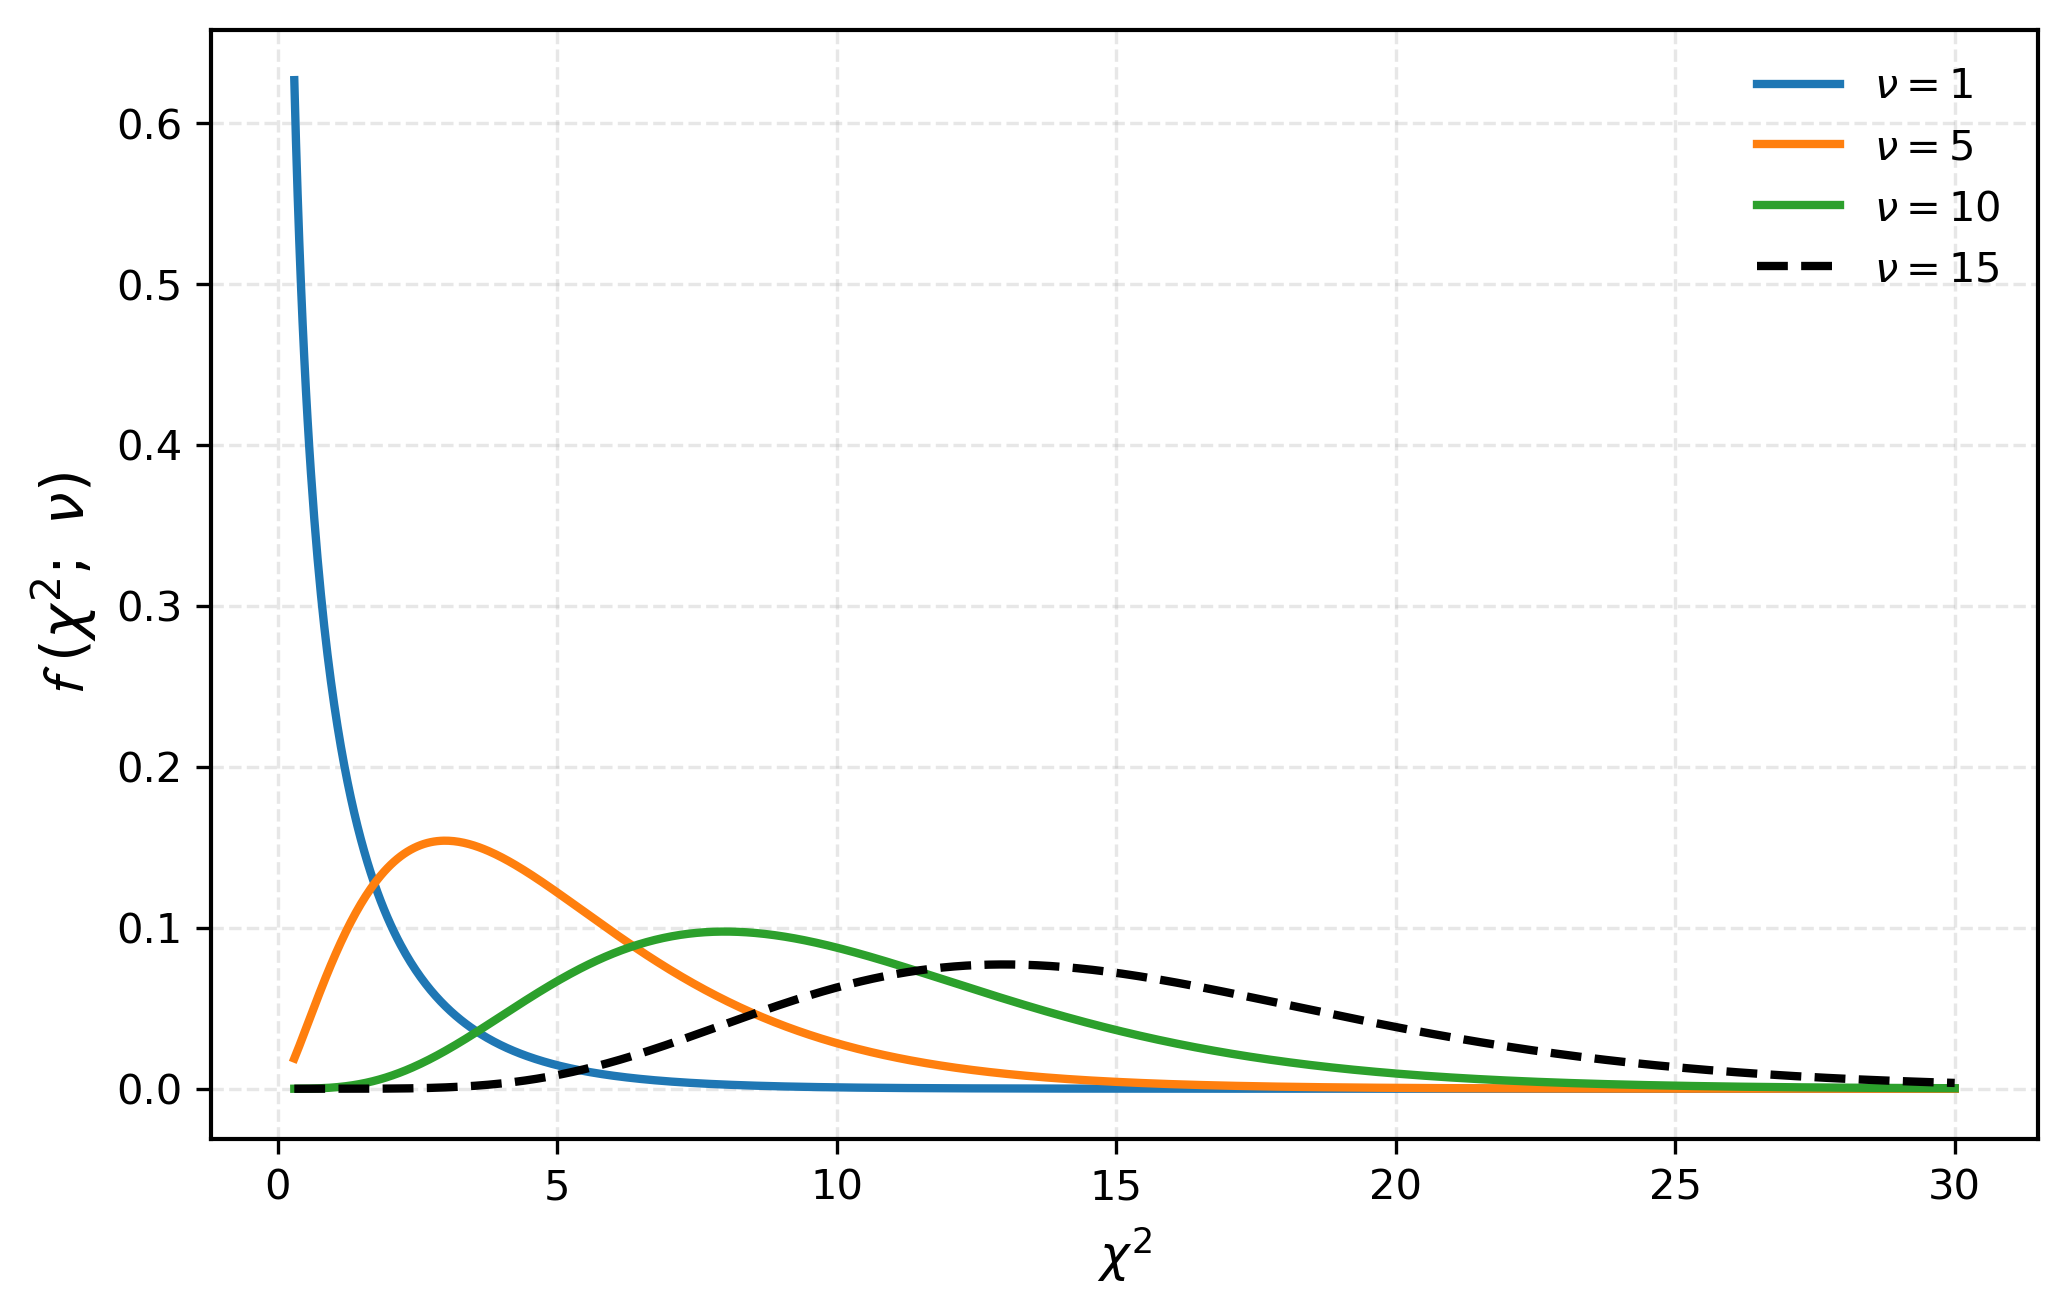
\includegraphics[width=0.7\textwidth]{figures/chapter4/chi2_distribution.png}
    \caption{Representation of the $chi^{2}$ distribution, for a particular value of the degrees of freedom ($\nu = 10$).}
    \label{fig:chi2_distribution}
\end{figure}

\newpage

\section{Parametric and non-parametric}

Parametric and non-parametric

\begin{enumerate}

\item \textbf{Student’s *t*-Test (One-Sample and Two-Sample)}\\
Introduced by William S. Gosset under the pseudonym “Student” in his seminal paper \cite{student1908}, this test allows inference on population means when the standard deviation is unknown and the sample size is small. The two-sample version compares the means of two independent groups under assumptions of normality and equal variances.\\
\textit{Non-parametric alternative:} The \textbf{Mann–Whitney U test} (also called the Wilcoxon rank-sum test) for independent samples, and the \textbf{Wilcoxon signed-rank test} for paired or single-sample symmetry testing.

\item \textbf{Fisher’s Exact Test}\\
Formulated by R. A. Fisher in his 1935 treatise on experimental design \cite{fisher1935}, this exact test computes the hypergeometric probability of a given 2x2 contingency table under the null hypothesis of independence. It is particularly suited for small samples, where asymptotic methods like chi-squared tests may not be valid.\\
\textit{Non-parametric alternative:} The test is already exact and non-parametric; however, \textbf{Barnard’s exact test} is sometimes proposed as a more powerful alternative in small-sample settings.

\item \textbf{Analysis of Variance (ANOVA)}\\
Fisher also introduced ANOVA in his earlier work \cite{fisher1925}, laying the foundation for modern experimental statistics. ANOVA decomposes total variation into between-group and within-group components, enabling testing of the equality of multiple means.\\
\textit{Non-parametric alternative:} The \textbf{Kruskal–Wallis H test}, which operates on ranks rather than means, is used when ANOVA assumptions (e.g., normality or homoscedasticity) are violated.

\item \textbf{Chi-Squared Test}\\
Originally proposed by Karl Pearson in 1900 \cite{pearson1900}, the chi-squared test evaluates how observed frequencies compare to expected frequencies under a null model of independence or goodness-of-fit. It is widely used in contingency table analysis and categorical data testing.\\
\textit{Non-parametric alternative:} While the chi-squared test is non-parametric in principle, \textbf{Fisher’s exact test} is often preferred for 2x2 tables with small expected counts.

\item \textbf{Welch’s *t*-Test (Unequal Variance Version)}\\
To address the limitations of assuming equal variances in the classical *t*-test, Welch proposed a generalization in 1947 \cite{welch1947} that remains robust under heteroscedasticity. It uses a weighted estimate of variance and adjusts the degrees of freedom accordingly.\\
\textit{Non-parametric alternative:} The \textbf{Mann–Whitney U test} again serves as a distribution-free method for comparing central tendencies when variance assumptions fail.

\end{enumerate}

\newpage

\section{Comparing data and normalization}

Comparing data and normalization


% Chapter - Linear models and GLMs
\chapter{Linear models and GLMs}

\section{Simple linear regression}
Simple linear regression

\newpage

\section{Multiple linear regression}
Multiple linear regression.

\newpage

\section{Hypothesis testing in linear models}
Hypothesis testing in linear models.

\newpage

\section{Generalized Linear Models (GLMs)}
Generalized Linear Models (GLMs).

\newpage

\section{Logistic, Poisson, polynomial regression}
Logistic, Poisson, polynomial regression.



% Chapter - Introduction to bayesian probability
\chapter{Introduction to bayesian probability}

\section{Bayesian vs frequentist}

So far we have discussed probability and statistics assuming the \textit{frequentist} definition of probability. That is, we have implicitly assumed that the probability, that number we make up to represent uncertainty, can be defined just as a ratio of the number of times we get a specific result, and the total number of observations. In the classic example of the coins, that we used in Chapter 2 to define probability in the first place, we are assuming, for instance, that the coin is fair. In the frequentist interpretation, probability is defined as the long-run relative frequency of an event occurring. For example, in the case of a fair coin:

\[
P(\text{H}) = \lim_{n \to \infty} \frac{\text{Number of H in } n \text{ tosses}}{n} = 0.5
\]

This approach assumes repeated experiments and well-defined probabilities that do not change. But if we start tossing the same coin again and again, and encounter that the ration of heads and tails is significantly different than 0.5, maybe we should start question that first assumption in the first place. Frequentist statistics might say we don't have enough data yet. But can we make a meaningful guess using prior knowledge and observed data? \\

This way of understanding probability, as founded in some \textit{prior beliefs} that can be updated as new evidence comes available, is normally referred to as \textit{bayesian} approach, or bayesian definition. It was developed by Thomas Bayes, a British mathematician who worked primarily on [...]. Early mathematicians like Pascal and Fermat formalized the idea of quantifying uncertainty. Over time, two main schools emerged: the frequentists, who interpret probability as the long-run frequency of events, and the Bayesians, who interpret probability as a degree of belief or certainty about an event. Thomas Bayes introduced the idea of updating probabilities based on new evidence. His work was published posthumously and it was later popularized by Laplace, and it is nowadays referred as the \textit{Bayes’ theorem}. Both approaches offer useful perspectives for understanding and analyzing uncertainty.\\

The frequentist approach relies on repeating experiments many times and observing how often events occur to estimate probabilities. It treats probability as an objective property of the physical world. In contrast, Bayesian probability treats it as a subjective measure of belief, updated as new data arrives. This difference influences how we interpret data and make predictions, and understanding both is important for a well-rounded grasp of statistics.\\

Frequentist methods often focus on long-run behaviour, like estimating probabilities from observed data or constructing confidence intervals. Bayesian methods combine prior knowledge (beliefs before seeing data) with observed data to update our understanding. In practice, both methods are used and combined and depending on the problem context.\\

\newpage

\section{The Bayes' Rule}

The second one — working backwards from results to reasons, purely, inferential — is what Bayes’ Theorem is all about. It’s how we reconstruct from data the underlaying phenomenology. From now on, w we will ask not only what is the probability for some event to take place, but what is the probability of that event happening \textit{given that} some other phenomena, some hypothesized scenario, is already taking place.\\

Bayes’ theorem appears often in biological sciences and medical tests, search engines, and in most data analysis problems when experimental results requiere interpretation and inference. It’s the engine behind how we learn from evidence, and once we understand it, we will start seeing it everywhere — from everyday decisions to machine learning. Its mathematical form can be written as follows. The \textit{conditional}, or \textit{posterior} probability of observing some some event $E$ happening, given some \textit{prior} knowledge, or hypothesis $H$ was true, is given by:

\begin{equation}
P(E|H) = \frac{P(H|E) \cdot P(H)}{P(E)}
\end{equation}

Where:
\begin{itemize}
  \item $P(E|H)$ is the probability of event $E$ given that $H$ has occurred (the \textbf{posterior}).
  \item $P(H|E)$ is the probability of event $E$ given $H$ (the \textbf{likelihood}).
  \item $P(H)$ is the probability of $H$ before seeing $E$ (the \textbf{prior}).
  \item $P(E)$ is the total — also called \textit{marginal} — probability of $E$ occurring (the \textbf{evidence}).
\end{itemize}

With bayesian probability we face now a complete different perspective. Bayesian probability treats probability as a degree of belief or confidence in a hypothesis. Rather than only relying on infinite repeated experiments, it allows us to update our beliefs in light of new evidence. Unlike the frequentist approach, we can incorporate prior information and handle small datasets. Bayes’ Rule provides the mechanism for updating beliefs.\\

Let's illustrate this with an example. Imagine we are given two dice, let's call them $D_1$ and $D_2$. The first one, $D_1$, is a far dice, and hence the probability of rolling any of the faces is uniformly distributed, all with probability $\frac{1}{6}$. But $D_2$ is biased, such that the probability of rolling a 6 is almost half the times. We can write the likelihoods of rolling a 6 in both cases, in the following way:
\begin{itemize}
  \item Dice 1 is \textbf{fair}, so $P(6|D_1) = \frac{1}{6}$.
  \item Dice 2 is \textbf{biased}, so $P(6|D_2) = \frac{1}{2}$.
\end{itemize}

We randomly pick one die, with no reason to favor either. Since we have just two options, the probability of choosing blindly one or the other — we will call this the \textit{prior} probability — is
\[
P(D_1) = P(D_2) = \frac{1}{2}
\]

Then, after that choice is made, we roll the dice and get a 6. And here is the question: What are the chances that we picked the biased die? Let's carefully define the prior beliefs and likelihoods, so that we can apply the Bayes rule. Let:

\begin{itemize}
  \item $H_1$: You picked the fair die.
  \item $H_2$: You picked the biased die.
  \item $E$: You rolled a 6.
\end{itemize}

We want to find $P(H_2 | E)$ — the probability that the die is biased given that we rolled a 6.\\

Using Bayes’ Theorem:

\[
P(H_2 | E) = \frac{P(E | H_2) \cdot P(H_2)}{P(S)}
\]

First, we calculate the marginal probability $P(E)$ — the overall chance of rolling a 6:

\[
P(E) = P(E | D_1) \cdot P(H_1) + P(E | D_2) \cdot P(H_2) = \frac{1}{6} \cdot \frac{1}{2} + \frac{1}{2} \cdot \frac{1}{2}
= \frac{1}{12} + \frac{1}{4} = \frac{1}{3}
\]

Now apply Bayes' Theorem:

\[
P(H_2 | E) = \frac{\frac{1}{2} \cdot \frac{1}{2}}{\frac{1}{3}} = \frac{1}{4} \div \frac{1}{3} = \frac{3}{4}
\]\\

Even though both dice had the same chance of being picked, rolling a 6 strongly points to the biased die. Bayes’ Theorem helped us turn a gut feeling into a solid number: a \textbf{75\% chance} that the die was biased. Bayes’ Theorem isn’t just math — it’s a mindset. It’s how we learn, adapt, and update our understanding when the world surprises us. Once you see it in action, it becomes a natural way to think about uncertainty and evidence.

\begin{itemize}
    \item \textbf{Frequentist}: Probability as long-run frequency.
    \item \textbf{Bayesian}: Probability as belief, updated with evidence.
\end{itemize}

\newpage

\subsection*{Exercise 1: Biased Coin (Frequentist)}
A coin is tossed 100 times and lands heads 56 times. Estimate the probability of heads using the frequentist approach.

\subsubsection*{Solution}
In the frequentist viewpoint, probability means the proportion of times an event happens in many repeated trials. Since the coin was tossed 100 times, we look at how often heads occurred to estimate its probability.

The estimated probability of heads is:
\[
P(\text{heads}) = \frac{\text{Number of heads}}{\text{Total tosses}} = \frac{56}{100} = 0.56
\]
This means we expect heads about 56\% of the time if the coin were tossed many more times.

\subsection*{Exercise 2: Bayesian Update (Bayes' Theorem)}
Suppose a disease affects 1\% of a population. A test detects the disease correctly 99\% of the time, but has a 5\% false positive rate. What is the probability that someone who tested positive actually has the disease?

\subsubsection*{Solution}
Bayesian probability helps us update our beliefs based on evidence. Here, we want to find the chance a person actually has the disease, given they tested positive.

Let's define events:
\begin{itemize}
    \item $D$: the person has the disease
    \item $T$: the test result is positive
\end{itemize}

We know from the problem:
\[
P(D) = 0.01 \quad\text{(1\% have the disease)}
\]
\[
P(\neg D) = 0.99 \quad\text{(99\% do not have it)}
\]
\[
P(T | D) = 0.99 \quad\text{(test is positive if disease present)}
\]
\[
P(T | \neg D) = 0.05 \quad\text{(5\% false positive rate)}
\]

Bayes’ theorem tells us:
\[
P(D | T) = \frac{P(T|D)P(D)}{P(T|D)P(D) + P(T|\neg D)P(\neg D)}
\]
This formula combines the likelihood of testing positive if diseased, weighted by how common the disease is, versus testing positive if not diseased.

Calculating:
\[
P(D | T) = \frac{0.99 \times 0.01}{0.99 \times 0.01 + 0.05 \times 0.99} = \frac{0.0099}{0.0099 + 0.0495} = \frac{0.0099}{0.0594} \approx 0.1667
\]

So, even if the test is positive, there is about a 16.7\% chance the person actually has the disease. This happens because the disease is rare, and false positives, while uncommon, happen more frequently.

\subsection*{Exercise 3: Confidence Interval (Frequentist)}
You roll a die 60 times and get the number 4 exactly 8 times. Construct a 95\% confidence interval for the probability of rolling a 4.

\subsubsection*{Solution}
A confidence interval gives a range where we expect the true probability to lie, based on our data.

First, calculate the observed probability:
\[
\hat{p} = \frac{8}{60} = 0.1333
\]

The standard error (SE) measures uncertainty in this estimate:
\[
\text{SE} = \sqrt{\frac{\hat{p}(1 - \hat{p})}{n}} = \sqrt{\frac{0.1333 \times 0.8667}{60}} \approx 0.0438
\]

For a 95\% confidence level, we use a multiplier $z=1.96$ (from the normal distribution).

The confidence interval is:
\[
\hat{p} \pm z \cdot \text{SE} = 0.1333 \pm 1.96 \times 0.0438 \approx 0.1333 \pm 0.0859
\]

This gives:
\[
(0.0474, 0.2192)
\]

Interpretation: If we repeated this experiment many times, 95\% of such intervals would contain the true probability of rolling a 4.

\newpage

\section{Bayesian vs frequentist}
Bayesian vs frequentist.

\newpage

\section{Computing posteriors}
Computing posteriors.



% Chapter - Introduction to Markov processes
\chapter{Introduction to Markov processes}

\section{Stochasticity and Markov processes}

The world around us is full of uncertainty. Facing questions like, will it rain tomorrow? Will a cell divide or die? Will a water drop fall in the same place after some time, or somewhere near? In many cases, the best we can do is talk in terms of probabilities — not certainties. This is where the idea of \textit{stochasticity} comes again, and why mathematicians of the 20th century deeply revisited its meaning. Stochasticity normally means randomness. From now on, we will define a stochastic process as a system that evolves over time in a way that involves some degree of randomness. Instead of asking, “What exactly will happen?” we ask, “What is likely to happen?”\\

Stochasticity means randomness or unpredictability in a system, as we have seen in previous chapters. But from now on, and following the work of mathematicians like Markov in the early 20th century, we will address it with a bit more subtlety. Now we will think about \textit{stochasticity} as randomness or unpredictability in a system, in opposition to deterministic systems, where future states are exactly determined by current conditions, stochastic systems incorporate randomness, making their outcomes probabilistic. Understanding stochasticity helps in modeling real-world phenomena where uncertainty is inherent, such as stock prices, weather, or population dynamics.\\

Even though the study of chance and probability can be trace to very ancient roots, as we have seen in previous chapter, \textit{stochasticity} as randomness or unpredictability in a system, in opposition to deterministic systems, began in the early 20th century, as mathematicians sought to model systems evolving randomly over time. Early work by Andrey Markov introduced Markov chains—models where the future depends only on the present state, not the past history. These models became fundamental in fields such as physics, biology, economics, and computer science for understanding complex systems affected by randomness. Over time, stochastic processes have grown into a broad discipline, providing tools for predicting and analyzing uncertain, evolving phenomena.\\

Markov processes are a class of stochastic models with the “memoryless” property—the future state depends only on the current state. This simplification makes analysis feasible and is surprisingly accurate for many systems. Markov chains are used in algorithms, queueing theory, genetics, and many other fields to describe how systems evolve step-by-step in time.\\

Many systems in nature and society follow patterns, but with noise, surprises, or variability. Markov models give us a way to describe and work with such systems — mathematically and intuitively. Imagine you're trying to predict the weather. If it’s sunny today, what are the chances it’ll be sunny tomorrow? What if it was rainy? Markov models help us answer these kinds of questions using a simple but powerful idea:\\

\textbf{The future depends only on the present — not the past.}\\

This is called the \textbf{Markov property}. A Markov model is a way to describe systems that move between states (like "sunny", "rainy", or "cloudy") with certain probabilities. Markov models are useful when things change over time in a somewhat random, yet patterned, way. Think of weather patterns, stock market movements, DNA sequences, pages people click on in a website, as examples. Even if we can’t predict everything perfectly, we can model how likely one thing is to follow another.\\

The key ingredients of a Markov model are:
\begin{itemize}
  \item A list of possible \textbf{states} (e.g., sunny, rainy), we will write as vectors.
  \item A \textbf{transition matrix}, encoding the probabilities of moving from one state to another.
\end{itemize}

Let's illustrate with a simple example. Let's try to predict weather in the following day, assuming stochasticity and knowledge of the previous states. For simplicity let’s say the weather can be either sunny ($S$) or rainy ($R$). And based on past data, we know:

\[
\text{Transition Matrix} =
\begin{bmatrix}
P(\text{Sunny} \rightarrow \text{Sunny}) & P(\text{Sunny} \rightarrow \text{Rainy}) \\
P(\text{Rainy} \rightarrow \text{Sunny}) & P(\text{Rainy} \rightarrow \text{Rainy})
\end{bmatrix}
=
\begin{bmatrix}
0.8 & 0.2 \\
0.4 & 0.6
\end{bmatrix}
\]

This means:
\begin{itemize}
  \item If today is Sunny, there's an 80\% chance tomorrow will also be Sunny, and 20\% chance of Rain.
  \item If today is Rainy, there's a 40\% chance it clears up, and a 60\% chance it stays rainy.
\end{itemize}

Suppose today is Sunny. We can represent our current state as a vector:

\[
\text{Today} = \begin{bmatrix} 1 & 0 \end{bmatrix}
\]

Then tomorrow’s prediction is:

\[
\text{Tomorrow} = \text{Today} \times \text{Transition Matrix} = 
\begin{bmatrix} 1 & 0 \end{bmatrix} \times
\begin{bmatrix}
0.8 & 0.2 \\
0.4 & 0.6
\end{bmatrix}
=
\begin{bmatrix}
0.8 & 0.2
\end{bmatrix}
\]

So there's an 80\% chance of Sun, 20\% chance of Rain tomorrow.\\

Markov models help us make predictions, model uncertainty, and understand patterns in time-based data. They are a stepping stone to more complex tools like Hidden Markov Models (HMMs), used in speech recognition, bioinformatics, and more [...].\\

Markov models are simple but powerful tools. They help us model systems that evolve over time, assuming that the next state only depends on the current one. Whether you’re analyzing text, tracking a robot, or predicting rain, the Markov assumption can be surprisingly useful [...].

\newpage

\subsection*{Exercise 1: Simple Random Walk}
A person starts at position 0 and at each step moves +1 or -1 with equal probability. What is the expected position after 10 steps?

\subsubsection*{Solution}
At each step, the person moves either forward (+1) or backward (-1) with equal chance 0.5. Because the steps are symmetric, the expected value (average position) after each step is zero.

Let $X_i$ represent the step at time $i$, which is +1 or -1, each with probability 0.5.

The total position after 10 steps is:
\[
S = \sum_{i=1}^{10} X_i
\]

The expectation is linear:
\[
\mathbb{E}[S] = \sum_{i=1}^{10} \mathbb{E}[X_i]
\]

Since each step is equally likely +1 or -1:
\[
\mathbb{E}[X_i] = (0.5)(+1) + (0.5)(-1) = 0
\]

Thus:
\[
\mathbb{E}[S] = 10 \times 0 = 0
\]

The expected position after 10 steps is 0, meaning the walk is equally likely to be positive or negative on average.

\subsection*{Exercise 2: Markov Chain Transition}
Given a Markov chain with states $A$, $B$, and the following transition matrix:
\[
P = \begin{bmatrix}
0.6 & 0.4 \\
0.3 & 0.7 \\
\end{bmatrix}
\]
If the initial state vector is $\pi_0 = [1\ 0]$ (starts at $A$), what is the state distribution after one and two steps?

\subsubsection*{Solution}
The transition matrix $P$ gives the probabilities of moving from one state to another in one step.

For example, the first row means:
- From state $A$, stay in $A$ with probability 0.6,
- Move to $B$ with probability 0.4.

The initial vector $\pi_0 = [1\ 0]$ means the system starts definitely in state $A$.

To find the state distribution after one step:
\[
\pi_1 = \pi_0 P = [1\ 0] \times \begin{bmatrix}0.6 & 0.4 \\ 0.3 & 0.7\end{bmatrix} = [0.6\ 0.4]
\]
This means after one step, there's a 60\% chance the system is in state $A$ and 40\% chance it is in $B$.

After two steps, multiply again:
\[
\pi_2 = \pi_1 P = [0.6\ 0.4] \times \begin{bmatrix}0.6 & 0.4 \\ 0.3 & 0.7\end{bmatrix}
\]
Calculate each element:
\[
\pi_2(A) = 0.6 \times 0.6 + 0.4 \times 0.3 = 0.36 + 0.12 = 0.48
\]
\[
\pi_2(B) = 0.6 \times 0.4 + 0.4 \times 0.7 = 0.24 + 0.28 = 0.52
\]

So after two steps, the system is in state $A$ with probability 48\%, and in $B$ with 52\%.

\subsection*{Exercise 3: Absorbing State}
A Markov chain has three states: 1 (start), 2 (intermediate), 3 (absorbing). The transition matrix is:
\[
P = \begin{bmatrix}
0 & 1 & 0 \\
0.5 & 0 & 0.5 \\
0 & 0 & 1 \\
\end{bmatrix}
\]
If the system starts in state 1, what is the probability it ends in state 3?

\subsubsection*{Solution}
An absorbing state is one where once entered, the system stays forever. Here, state 3 is absorbing because it transitions to itself with probability 1.

We want the probability that starting from state 1, the process eventually reaches state 3.

From state 1:
- It always moves to state 2 (probability 1).

From state 2:
- With probability 0.5, it moves to state 1,
- With probability 0.5, it moves to absorbing state 3.

Because from state 2 there is a chance to return to 1, the system may loop between states 1 and 2 many times before reaching 3.

Define:
\[
p = \text{probability of eventually reaching 3 starting from 1}
\]
\[
q = \text{probability of eventually reaching 3 starting from 2}
\]

From state 1, since it always goes to 2:
\[
p = q
\]

From state 2:
\[
q = 0.5 \times 1 + 0.5 \times p
\]
The $0.5 \times 1$ is probability of going directly to absorbing 3, which is certain to stay there (hence probability 1 of absorption).

Substitute $p = q$:
\[
q = 0.5 + 0.5 q
\Rightarrow 0.5 q = 0.5
\Rightarrow q = 1
\]

So $p = 1$ also.

This means the system will reach the absorbing state 3 with probability 1 (certainty), though it might take several steps cycling between 1 and 2 first.

\newpage

\section{Markov chains}
Markov chains.

\newpage

\section{Hidden Markov models}
Hidden Markov models.

\newpage

\appendix

% Chapter: Vectors and matrices
\chapter{Vectors and matrices: a quick review}

\section{Vectors and their properties}

\section{Matrices and linear transformations}

\section{Basic algebraic operations}

\newpage

% Chapter: Derivatives
\chapter{Functions and derivatives: a quick review}

\section{From curves to calculus: functions}

\section{The idea of change, slope and minima}

\section{Derivatives}

\newpage

% Chapter: Integrals
\chapter{Integrals: a quick review}

\section{Indefinite integral as antiderivative}

\section{Define definite integral as area under a curve}

\section{The fundamental theorem of calculus}

% Chapter: Fourier series
\chapter{Fourier series: a quick review}

\section{Introduction to periodic functions}

\section{Orthogonality and approximating functions}

\section{Conditions of convergence}

\section{Applications: the heat equation}

\backmatter
 
\begin{thebibliography}{999}

\bibitem{spiegelhalter2019art} 
David Spiegelhalter. 
\textit{The Art of Statistics: How to Learn from Data}. 
Basic Books, 2019.

\bibitem{degroot2012probability}
Morris H. DeGroot and Mark J. Schervish.
\textit{Probability and Statistics} (4th ed.).
Pearson, 2012.

\bibitem{mcfadden2011philosophy}
J. A. F. McFadden.
\textit{The Philosophy of Statistics}.
Wiley-Blackwell, 2011.

\bibitem{openintro2025}
M. Diez, D. Barr, and Çetinkaya-Rundel.
\textit{OpenIntro Statistics}.
OpenIntro, 2025.

\bibitem{pishronik2014introduction}
Hossein Pishro-Nik.
\textit{Introduction to Probability, Statistics and Random Processes}.
Kappa Research LLC, 2014.

\bibitem{student1908}
Student. (1908). *The probable error of a mean*. Biometrika, 6(1), 1–25.

\bibitem{fisher1925}
Fisher, R. A. (1925). *Statistical Methods for Research Workers*. Edinburgh: Oliver and Boyd.

\bibitem{fisher1935}
Fisher, R. A. (1935). *The Design of Experiments*. Edinburgh: Oliver and Boyd.

\bibitem{pearson1900}
Pearson, K. (1900). *On the criterion that a given system of deviations from the probable in the case of a correlated system of variables is such that it can be reasonably supposed to have arisen from random sampling*. Philosophical Magazine Series 5, 50(302), 157–175.

\bibitem{welch1947}
Welch, B. L. (1947). *The generalization of "Student’s" problem when several different population variances are involved*. Biometrika, 34(1–2), 28–35.

\bibitem{yates1934}
Yates, F. (1934). *Contingency tables involving small numbers and the $\chi^2$ test*. Supplement to the Journal of the Royal Statistical Society, 1(2), 217–235.

\bibitem{greenwood1911}
Greenwood, M., \& Yule, G. U. (1911). *An inquiry into the nature of frequency distributions representative of multiple happenings with particular reference to the occurrence of multiple attacks of disease or of repeated accidents*. Journal of the Royal Statistical Society, 83(2), 255–279.

\end{thebibliography}

\end{document}
